%!Mode:: "TeX:UTF-8"
%!TEX program = xelatex

\documentclass[UTF-8]{progbookcn}
\usepackage{graphicx}
\usepackage[dvipsnames]{xcolor}
\usepackage{wrapfig}
\usepackage{enumerate}
\usepackage{amsmath,mathrsfs,amsfonts}
\usepackage{amssymb}
\usepackage{tabularx}
\usepackage{booktabs}
\usepackage{colortbl}
\usepackage{multirow,makecell}
\usepackage{multicol}
\usepackage{ulem} % \uline
\usepackage{listings}
\usepackage{tikz}
\usepackage{tcolorbox}
\usepackage{fontawesome5}
\usepackage{lipsum}
\usepackage{overpic}
\usepackage[normalem]{ulem}
\usepackage{footnote}
\usepackage{booktabs}
\usepackage{bm}
\usepackage{threeparttable}
\usepackage{CJK}
\usepackage{longtable}
\usepackage{cite}
\useunder{\uline}{\ul}{}

\graphicspath{{figs/}}

%%%%%%%%%%%%%%%%%%%%%%%%%%%%%%%%%%%%%%%%
%% beginning of the book
%% 文档开始
%%%%%%%%%%%%%%%%%%%%%%%%%%%%%%%%%%%%%%%%

\setmainfont{Times New Roman}



\usepackage{amsmath}

\newtheorem{example}{例}[chapter]         % 整体编号
\newtheorem{algorithm}{算法}[chapter]
\newtheorem{theorem}{定理}[chapter]  % 按 section 编号

\newtheorem{axiom}{公理}[chapter]
\newtheorem{property}{性质}[chapter]
\newtheorem{proposition}{命题}[chapter]
\newtheorem{lemma}{引理}[chapter]
\newtheorem{corollary}{推论}[chapter]
\newtheorem{remark}{注解}[chapter]
\newtheorem{condition}{条件}[chapter]
\newtheorem{conclusion}{结论}[chapter]
\newtheorem{assumption}{假设}[chapter]
%\newtheorem{proof}{证明}[section]
\newtheorem{definition}{定义}[chapter]
%\newenvironment{definition}{{\noindent\textbf{定义:}}}{\hfill $\square$\par}
\newenvironment{proof}{{\noindent\textbf{证明:}}}{\hfill $\square$\par}

\newenvironment{cmd}{\fontfamily{Kai}\selectfont}






\begin{document}

%% title page
\begin{titlepage}
  \vspace*{25ex}

  \hspace{0.05\textwidth}\begin{minipage}{.9\textwidth}
    \flushright

    %%中文书名
    {\zihao{1}\textbf{基于MSVL的神经网络框架}}

    \rule{\linewidth}{.5pt}

    \vspace{2ex}

    %% 英文书名
    {\zihao{2}\textsf{Framework for Neural Networks Based on MSVL}} \\

    \vspace{20ex}

    %% 作者
    {\zihao{4}\textit{冯哲}}~~~~~~~~~~~~~~~~~~~

    \vspace{20ex}

  \end{minipage}

  \vfill

  \centering
  {\zihao{4} \textsf{西安电子科技大学} ~$\bullet$~ \textsf{ICTT}}
\end{titlepage}
\thispagestyle{empty}


\frontmatter


\centerline{\Large\bf{符\hspace{0.5em}号\hspace{0.5em}对\hspace{0.5em}照\hspace{0.5em}表}\vspace{1em}}
\begin{table}[!ht]
%\label{}
%\setlength{\tabcolsep}{7mm}{
\begin{tabular}{l|l}
\multicolumn{2}{l}{~~~~~~~~~~~~~~~~~~\textbf{数相关符号}}\\ \hline
\textbf{符号}\hspace{12em} & \textbf{含义}          \\  \hline
$x$                                & 标量 \\
$\bm{x}$                         & 向量  \\
$\bm{X}$                         & 矩阵     \\
$X$                         & 张量       \\ \hline
\multicolumn{2}{l}{~~~~~~~~~~~~~~~~~~}\\
\multicolumn{2}{l}{~~~~~~~~~~~~~~~~~~\textbf{操作符相关符号}}\\ \hline
\textbf{符号}\hspace{12em} & \textbf{含义}          \\  \hline
$(\cdot)^T$                  & 向量或者矩阵的转置 \\
$\odot$                         & 按元素相乘  \\
$\|\cdot\|_p$                         & $L_p$范数     \\
$\|\cdot\|$                         & $L_2$范数     \\
$\sum$                         & 连加     \\
$\prod$                         & 连乘     \\
\hline\multicolumn{2}{l}{~~~~~~~~~~~~~~~~~~}\\
\multicolumn{2}{l}{~~~~~~~~~~~~~~~~~~\textbf{函数相关符号}}\\ \hline
\textbf{符号}\hspace{12em} & \textbf{含义}          \\  \hline
$f(\cdot)$                                & 函数 \\
$\log(\cdot)$                         & 自然对数函数  \\
$\exp(\cdot)$                         & 指数函数     \\
\hline \multicolumn{2}{l}{~~~~~~~~~~~~~~~~~~}\\
\multicolumn{2}{l}{~~~~~~~~~~~~~~~~~~\textbf{导数和梯度相关符号}}\\ \hline
\textbf{符号}\hspace{12em} & \textbf{含义}          \\  \hline
$\frac{dy}{dx}$                                & $y$关于$x$的导数 \\
$\frac{\partial y}{\partial x}$                         &  $y$关于$x$的偏导 \\
$\nabla_{\bm{x}} y$                         & $y$关于向量$\bm{x}$的梯度 \\
\hline\multicolumn{2}{l}{~~~~~~~~~~~~~~~~~~}\\
\multicolumn{2}{l}{~~~~~~~~~~~~~~~~~~\textbf{概率统计相关符号}}\\ \hline
\textbf{符号}\hspace{12em} & \textbf{含义}          \\  \hline
$\cdot \sim N(\mu, \sigma^2)$                         & 随机变量$\cdot$服从高斯分布   \\
$\cdot \sim U(-\alpha,~ \alpha)$                       & 随机变量$\cdot$服从均匀分布   \\
$E(\cdot)$                                & 随机变量$\cdot$的数学期望 \\
$Var(\cdot)$                                & 随机变量$\cdot$的方差 \\ \hline
\end{tabular}%}
\end{table}





%% 目录
\clearpage
{
  \hypersetup{hidelinks}
  \tableofcontents
}


\mainmatter


\part{算法理论基础}
\chapter{神经网络介绍}

人工神经网络(Artificial Neural Network,ANN),简称神经网络(Neural Network,NN)或类神经网络,在机器学习和认知科学领域,是一种模仿生物神经网络的结构和功能的数学模型或计算模型,用于对函数进行估计或近似\cite{DBLP:journals/robotica/Andrew99j}。神经网络由大量的神经元联结进行计算。大多数情况下神经网络能在外界信息的基础上改变内部结构,是一种自适应系统,通俗的讲就是具备学习功能\cite{DBLP:journals/nn/SchiffmannG93}。现代神经网络是一种非线性统计性数据建模工具,神经网络通常是通过一个基于数学统计学类型的学习方法得以优化,所以也是数学统计学方法的一种实际应用,通过统计学的标准数学方法我们能够得到大量的可以用函数来表达的局部结构空间,另一方面在人工智能学的人工感知领域,我们通过数学统计学的应用可以来做人工感知方面的决定问题,一般这种方法比起正式的逻辑学推理演算更具有优势\cite{DBLP:journals/ijon/PrietoPORPOR16}。

\section{神经元}
对于神经元的研究由来已久,1904年生物学家就已经知晓了神经元的组成结构。一个神经元通常具有多个树突,主要用来接受传入信息;而轴突只有一条,轴突尾端有许多轴突末梢可以给其他多个神经元传递信息。轴突末梢跟其他神经元的树突产生连接,从而传递信号。这个连接的位置在生物学上叫做“突触”\cite{Ram}。

1943年,心理学家McCulloch和数学家Pitts参考了生物神经元的结构,发表了抽象的神经元模型MP。神经元模型是一个包含输入,输出与计算功能的模型。输入可以类比为神经元的树突,而输出可以类比为神经元的轴突,计算则可以类比为细胞核\cite{DBLP:books/ox/90/McCullochP90}。




图(\ref{NU})是一个典型的神经元模型:包含有3个输入[$x_1,x_2,x_3$],1个输出[$y$],以及2个计算功能(求和$\sum$以及非线性函数sgn见公式(\ref{sgn}))。 注意中间的连线。这些线称为“连接”。每个上有一个“权值”。其中的偏置$b$也可以看成是一个输入神经元值为1的一个“连接”上的“权值”。
 \begin{equation}\label{sgn}
    \text{sgn}(x) = \begin{cases}
                   ~~0, & \mbox{if } z<0 \\
                   ~~1, & \mbox{otherwise}.
                 \end{cases}
 \end{equation}

 \begin{figure}[!h]
  \centering
  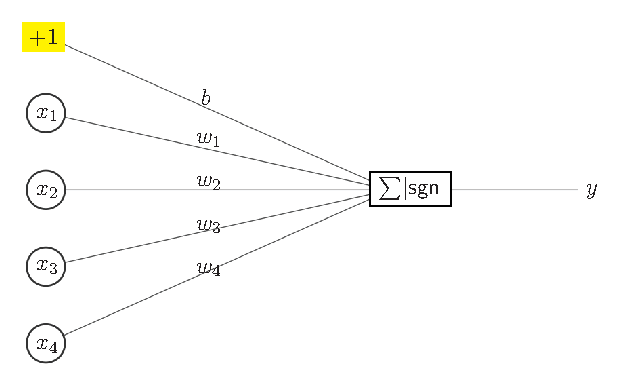
\includegraphics[width=0.4\textwidth]{tu1.eps}
  \caption{神经元(MP)结构}\label{NU}
\end{figure}

将神经元结构图中的所有变量用符号表示,并且写出输出的计算公式的话,就是公式(\ref{ES})。
 \begin{equation}\label{ES}
    y = \text{sgn}(w_1x_1+w_2x_2+w_3x_3+b)
 \end{equation}




一个神经网络的训练算法就是让权重的值调整到最佳,以使得整个网络的预测效果最好。当用“神经元”组成网络以后,描述网络中的某个“神经元”时,我们更多地会用“单元”(unit)来指代。同时由于神经网络的表现形式是一个有向图,有时也会用“节点”(node)来表达同样的意思。


神经元模型的使用可以这样理解:存在一个数据,称之为样本。样本有五个属性,其中四个属性已知,一个属性未知。通过四个已知属性预测未知属性。具体办法就是使用神经元的公式进行计算。四个已知属性的值是$x_1,x_2,x_3,x_4$,未知属性的值是$y$。$y$通过公式计算出来。这里,已知的属性称之为特征,未知的属性称之为目标。假设特征与目标之间确实是线性关系,并且得到表示这个关系的权值$w_1,w_2,w_3,w_4$。那么,便可通过神经元模型预测新样本的目标。

起初由于计算机计算能力以及权值都是预先设置的等原因,神经元是不能学习的,直到接近10年后,第一个真正意义的神经网络才诞生。

\section{单层神经网络}
1958年,计算科学家Rosenblatt提出了由两层神经元组成的神经网络。命名为“感知器”(Perceptron)感知器是当时首个可以学习的人工神经网络\cite{Rosenblatt58theperceptron:}。Rosenblatt现场演示了其学习识别简单图像的过程,在当时的社会引起了轰动。人们认为已经发现了智能的奥秘,许多学者和科研机构纷纷投入到神经网络的研究中。美国军方大力资助了神经网络的研究,并认为神经网络比“原子弹工程”更重要。这段时间直到1969年才结束,这个时期可以看作神经网络的第一次高潮。

在“感知器”中,有两个层次。分别是输入层和输出层。输入层里的“输入单元”只负责传输数据,不做计算。输出层里的“输出单元”则需要对前面一层的输入进行计算。把需要计算的层次称之为“计算层”,并把拥有一个计算层的网络称之为“单层神经网络”。假如要预测的目标不再是一个值,而是一个向量。那么可以在输出层再几个“输出单元”。

下图(\ref{fig:SNN})显示了带有八个输出单元的单层神经网络,其中输出单元$z_1$的计算公式如(\ref{Eq:1.2.1})。
\begin{equation}\label{Eq:1.2.1}
  z_1 = \text{sgn}(w_{01}+w_{11}x_1+w_{21}x_2+w_{31}x_3)
\end{equation}

%\begin{overpic}[width=0.35\textwidth]{tu2.eps}
%\put(0, 75.2){\huge\textcolor{white}{一}}
%\put(0, 75.3){\huge\textcolor{white}{一}}
%\put(0, 75.4){\huge\textcolor{white}{一}}
%\put(0, 75.5){\huge\textcolor{white}{一}}
%\put(0, 75.6){\huge\textcolor{white}{一}}
%\put(0, 75.7){\huge\textcolor{white}{一}}
%\put(0, 75.8){\huge\textcolor{white}{一}}
%\put(0, 75.9){\huge\textcolor{white}{一}}
%\put(0, 76){\huge\textcolor{white}{一}}
%\put(0, 76.1){\huge\textcolor{white}{一}}
%\put(0, 76.2){\huge\textcolor{white}{一}}
%\put(0, 76.3){\huge\textcolor{white}{一}}
%\put(0, 76.4){\huge\textcolor{white}{一}}
%\put(0, 76.5){\huge\textcolor{white}{一}}
%\put(0, 76.6){\huge\textcolor{white}{一}}
%\put(0, 76.7){\huge\textcolor{white}{一}}
%
%
%\put(1,73.9){\colorbox{yellow}{+1}}
%
%\put(2.4,62.2){\large $x_1$}
%\put(2.4,49.3){\large$x_2$}
%\put(2.4,36.4){\large$x_3$}
%\put(2.4,23.4){\large$x_4$}
%
%\put(60.5,94.5){\large $z_1$}
%\put(60.5,81.5){\large$z_2$}
%\put(60.5,68.5){\large$z_3$}
%\put(60.5,55.5){\large$z_4$}
%\put(60.5,42.6){\large $z_5$}
%\put(60.5,29.7){\large$z_6$}
%\put(60.5,16.8){\large$z_7$}
%\put(60.5,3.9){\large$z_8$}
%
%\put(30,85){$w_{01}$}
%\put(33,81){$w_{11}$}
%\put(40.5,81.5){$w_{21}$}
%\put(47.5,85.2){$w_{31}$}
%\put(55,90){$w_{41}$}
%\end{overpic}


\begin{figure}[!ht]
  \centering
  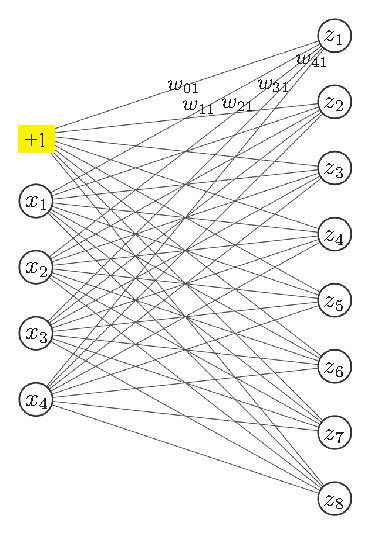
\includegraphics[width=0.36\textwidth]{tu2F.eps}
  \caption{单层神经网络结构}\label{fig:SNN}
\end{figure}

已知一个神经元的输出可以向多个神经元传递,因此$z_2$的计算公式(\ref{Eq:1.2.2})。

\begin{equation}\label{Eq:1.2.2}
  z_2 = \text{sgn}(w_{02}+w_{12}x_1+w_{22}x_2+w_{32}x_3)
\end{equation}

观察输出的计算公式,会发现这两个公式就是线性代数方程组。因此可以用矩阵乘法来表达这两个公式。例如,输入的变量是$[1, x_1,~x_2,~x_3,~x_4]$(代表由$1, x_1,~x_2,~x_3,~x_4$组成的行向量),用向量$\bm{x^T}$来表示。方程的左边是$[z_1,~z_2,~z_3,~z_4,~z_5,~z_6,~z_7,~z_8]$,用向量$\bm{z}$来表示。系数则是矩阵$\bm{W}$(5行8列的矩阵,排列形式与公式中的一样)。于是,输出公式可以改写成公式(\ref{Eq:1.2.3}):

\begin{equation}\label{Eq:1.2.3}
 \bm{z^T} = \text{sgn}(\bm{x^T}\bm{W})
\end{equation}


与神经元模型不同,感知器中的权值是通过训练得到的。感知器类似一个逻辑回归模型,可以做线性分类任务。可以用决策分界来形象的表达分类的效果。决策分界就是在二维的数据平面中划出一条直线,当数据的维度是3维的时候,就是划出一个平面,当数据的维度是n维时,就是划出一个n-1维的超平面。
下图(\ref{fig:perceptron})显示了在二维平面中划出决策分界的效果,也就是感知器的分类效果。

\begin{figure}[!ht]
  \centering
  \includegraphics[width=0.55\textwidth]{PerceptronOrigin.eps}
  \caption{单层神经网络(决策分界)}\label{fig:perceptron}
\end{figure}

感知器只能做简单的线性分类任务。但是当时的人们热情太过于高涨,并没有人清醒的认识到这点。于是,当人工智能领域的巨擘Minsky指出这点时,事态就发生了变化。Minsky在1969年出版了一本叫《Perceptron》的书,里面用详细的数学证明了感知器的弱点,尤其是感知器对XOR(异或)这样的简单分类任务都无法解决\cite{Pollack_bookreview:}。Minsky认为,如果将计算层增加到两层,计算量则过大,而且没有有效的学习算法。所以,他认为研究更深层的网络是没有价值的。由于Minsky的巨大影响力以及书中呈现的悲观态度,让很多学者和实验室纷纷放弃了神经网络的研究。神经网络的研究陷入了冰河期。这个时期又被称为“AI winter”。接近10年以后,对于两层神经网络的研究才带来神经网络的复苏。



\section{多层神经网络}
Minsky说过单层神经网络无法解决异或问题。但是当增加一个计算层以后,两层神经网络不仅可以解决异或问题,而且具有非常好的非线性分类效果。不过两层神经网络的计算是一个问题,没有一个较好的解法。

1986年,Rumelhar和Hinton等人提出了反向传播(Backpropagation,BP)算法,解决了两层神经网络所需要的复杂计算量问题,从而带动了业界使用两层神经网络研究的热潮\cite{BP}。

在两层神经网络中,不再使用sgn函数,而是使用平滑函数sigmoid。把此类函数也称作激活函数(active function)。事实上,神经网络的本质就是通过参数与激活函数来拟合特征与目标之间的真实函数关系。


与单层神经网络不同。理论证明,两层神经网络可以无限逼近任意连续函数。

机器学习模型训练的目的,就是使得参数尽可能的与真实的模型逼近。具体做法是这样的。首先给所有参数赋上随机值。我们使用这些随机生成的参数值,来预测训练数据中的样本。样本的预测目标为$y_p$,真实目标为$y$。那么,定义一个值$loss$,计算公式如式(\ref{Eq:1.3.1})。

\begin{equation}\label{Eq:1.3.1}
  loss = (y_p - y)^2
\end{equation}

这个值称之为损失(loss),我们的目标就是使对所有训练数据的损失和尽可能的小。下面的问题就是求:如何优化参数,能够让损失函数的值最小。

这个问题就被转化为一个优化问题。一个常用方法就是高等数学中的求导,但是这里的问题由于参数不止一个,求导后计算导数等于0的运算量很大,所以一般来说解决这个优化问题使用的是梯度下降算法。梯度下降算法每次计算参数在当前的梯度,然后让参数向着梯度的反方向前进一段距离,不断重复,直到梯度接近零时截止。一般这个时候,所有的参数恰好达到使损失函数达到一个最低值的状态。

在神经网络模型中,由于结构复杂,每次计算梯度的代价很大。因此还需要使用反向传播算法。反向传播算法是利用了神经网络的结构进行的计算。不一次计算所有参数的梯度,而是从后往前。首先计算输出层的梯度,然后是第二个参数矩阵的梯度,接着是中间层的梯度,再然后是第一个参数矩阵的梯度,最后是输入层的梯度。计算结束以后,所要的两个参数矩阵的梯度就都有了。

两层神经网络在多个地方的应用说明了其效用与价值。10年前困扰神经网络界的异或问题被轻松解决。神经网络在这个时候,已经可以发力于语音识别,图像识别,自动驾驶等多个领域。
\begin{figure}[!ht]%{5cm}
  \centering
  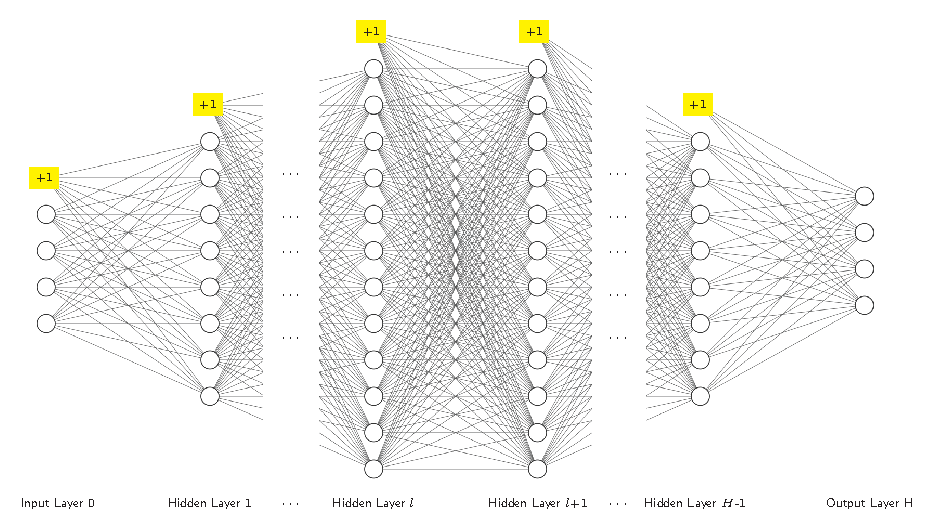
\includegraphics[width=0.88\textwidth]{NNF.eps}
  \caption{全连接神经网络结构}
  \label{fig:NNFrame}
\end{figure}




在被人摒弃的10年中,有几个学者仍然在坚持研究。这其中的棋手就是加拿大多伦多大学的Geoffery Hinton教授。2006年,Hinton在《Science》和相关期刊上发表了论文,首次提出了“深度信念网络”的概念\cite{DBLP:journals/neco/HintonOT06}。与传统的训练方式不同,“深度信念网络”有一个“预训练”(pre-training)的过程,这可以方便的让神经网络中的权值找到一个接近最优解的值,之后再使用“微调”(fine-tuning)技术来对整个网络进行优化训练。这两个技术的运用大幅度减少了训练多层神经网络的时间。他给多层神经网络相关的学习方法赋予了一个新名词--“深度学习”。在这之后,关于深度神经网络的研究与应用不断涌现。

在两层神经网络的输出层后面,继续添加层次。原来的输出层变成中间层,新加的层次成为新的输出层。所以可以得到图(\ref{fig:NNFrame})。依照这样的方式不断添加,我们可以得到更多层的多层神经网络。公式推导跟两层神经网络类似,使用矩阵运算仅仅是加一个公式。

与两层层神经网络不同。多层神经网络中的层数增加了很多。增加更多的层次有更深入的表示特征,以及更强的函数模拟能力。更深入的表示特征可以这样理解,随着网络的层数增加,每一层对于前一层次的抽象表示更深入。在神经网络中,每一层神经元学习到的是前一层神经元值的更抽象的表示。例如第一个隐藏层学习到的是“边缘”的特征,第二个隐藏层学习到的是由“边缘”组成的“形状”的特征,第三个隐藏层学习到的是由“形状”组成的“图案”的特征,最后的隐藏层学习到的是由“图案”组成的“目标”的特征。通过抽取更抽象的特征来对事物进行区分,从而获得更好的区分与分类能力。
%
%\newpage
%
%\begin{enumerate}
%  \item 统计学习方法-李航
%  \item 机器学习-周志华
%  \item 吴恩达(Andrew Ng)机器学习网课【这个是结合学习的网课,网上都有】
%  \item 机器学习实战-Peter Harrington【结合理论编程书目python】
%  \item Deep Learning(深度学习)-(花书)【进阶书目】
%  \item Pattern Recognition and Machine Learning【进阶书目】
%\end{enumerate}
%\newpage


\chapter{神经网络理论基础}

\section{神经网络激活函数}
激活函数是神经网络的一个重要组成部分。如果不用激活函数,在这种情况下,网络的每一层的输入都是上一层的线性输出,因此,无论该神经网络有多少层,最终的输出都是输入的线性组合,与没有隐藏层的效果相当,这种情况就是最原始的感知机。因此,需要引入非线性函数作为激活函数,这样深层神经网络才有意义,输出不再是输入的线性组合,就可以逼近任意函数\cite{DBLP:books/daglib/0040158}。本节给出五种比较常用的激活函数及其导函数。

\subsection{sigmoid\cite{DBLP:journals/mcss/Cybenko89}}
\begin{equation}\label{E11}
  \sigma(z) = \frac{1}{1+e^{-z}}
\end{equation}

\begin{equation}\label{E12}
  \sigma'(z) = \sigma(z)(1-\sigma(z))
\end{equation}



\subsection{tanh}
  \begin{equation}\label{E21}
    \sigma(z) = \frac{e^z-e^{-z}}{e^z+e^{-z}} = 1- \frac{2e^{-z}}{e^z + e^{-z}}
  \end{equation}
  \begin{equation}\label{E22}
    \sigma'(z) = 1-\sigma(z)^2
  \end{equation}


\subsection{relu\cite{Maas13rectifiernonlinearities}}
 \begin{equation}\label{E31}
    \sigma(z) = \begin{cases}
                   ~~0, & \mbox{if } z<0 \\
                   ~~z, & \mbox{otherwise}.
                 \end{cases}
 \end{equation}
 \begin{equation}\label{E32}
    \sigma'(z) = \begin{cases}
                   ~~0, & \mbox{if } z<0 \\
                   ~~1, & \mbox{otherwise}.
                 \end{cases}  \\
  \end{equation}


\subsection{leaky relu}
  \begin{equation}\label{E41}
    \sigma(z) = \begin{cases}
                   ~~z, & \mbox{if } z>0 \\
                   ~~az, & \mbox{otherwise}.
                 \end{cases}\\
  \end{equation} \centerline{~~~~~~~~~~~~~~~~~~~~~~~~~~~~~~~~~~~~~~~~~~~~其中$a$为斜率,又称倾斜因子。}
  \begin{equation}\label{E42}
    \sigma'(z) = \begin{cases}
                   ~~1, & \mbox{if } z>0 \\
                   ~~a, & \mbox{otherwise}.
                 \end{cases}\\
  \end{equation}

\subsection{softmax\cite{DBLP:journals/corr/abs-1905-10626}}

  \begin{equation}\label{E51}
  \text{第 i 个类目的概率,}\\
    p_i = a^{(N+1)}_i =\sigma(s^{(N+1)}_i)= \frac{e^{s^{(N+1)}_i}}{\sum_{j=1}^{K} e^{s^{(N+1)}_j}}
  \end{equation}
  $$
\delta_{ij}=
\begin{cases}
1& i=j\\
0& i\neq j
\end{cases}
$$
\begin{equation}\label{E52}
\frac{\partial p_i}{\partial s_j}=p_i(\delta_{ij}-p_j)
\end{equation}

\begin{proof} 公式(\ref{E52})\\
\indent ~~~~~~~~对softmax函数求导:
\begin{align*}
  &\frac{\partial p_i}{\partial s_j}=\frac{\partial\frac{e^{s_i}}{\sum_{k=1}^{N}e^{s_k}}}{\partial s_j}\\
  &f(x) = \frac{g(x)}{h(x)},~~~~~~~~~f'(x)=\frac{g'(x)h(x)-h'(x)g(x)}{h^2(x)}\\
  &g(x)=e^{s_i},~~~~~~~~~h(x)=\sum_{k=1}^{N}e^{s_k}\\
  &\text{当~}i=j~:\\
  &\frac{\partial\frac{e^{s_i}}{\sum_{k=1}^{N}e^{s_k}}}{\partial s_j}=\frac{e^{s_i} \sum_{k=1}^{N} e^{s_k}-e^{s_j}e^{s_i}}{\big(\sum_{k=1}^{N}e^{s_k}\big)^2}
  =\frac{e^{s_i}\big(\sum_{k=1}^{N}e^{s_k}-e^{s_j}\big)}{\big(\sum_{k=1}^{N}e^{s_k}\big)^2}
  =p_i(1-p_j)\\
  &\text{当~}i\neq j~:\\
  &\frac{\partial\frac{e^{s_i}}{\sum_{k=1}^{N}}}{\partial s_j}=\frac{0-e^{s_j}e^{s_i}}{\big(\sum_{k=1}^{N}e^{s_k}\big)^2}
  =-\frac{e^{s_i}}{\sum_{k=1}^{N}e^{s_k}}\frac{e^{s^j}}{\sum_{k=1}^{N}e^{s_k}}
  =-p_ip_j\\
  &\text{因此:}\\
  &\delta_{ij}=
\begin{cases}
1& i=j\\
0& i\neq j
\end{cases}\\
&\frac{\partial p_i}{\partial s_j}=p_i(\delta_{ij}-p_j)
\end{align*}
\end{proof}


\section{神经网络损失函数}
损失函数有助于优化神经网络的参数。训练神经网络的目标是通过优化神经网络的参数来最大程度地减少神经网络的损失。通过神经网络将目标值与预测值进行匹配,再经过损失函数就可以计算出损失。然后,我们使用梯度下降法来优化网络权重,以使损失最小化\cite{DBLP:books/daglib/0040158}。此节给出两种常用的损失函数及其导函数。
\subsection{Mean Square Error}
\begin{equation}\label{2.2.1.1}
  Loss(\bm{z},\bm{y}) =\frac{1}{2} \sum_{i=1}^{K}(z_i-y_i)^2
\end{equation}
\begin{equation}\label{2.2.1.2}
\frac{\partial Loss}{\partial \bm{z}}  = (\bm{z}-\bm{y})
\end{equation}
\subsection{Cross Entropy Loss\cite{DBLP:journals/corr/abs-1905-10626}}
\begin{equation}\label{2.2.1.3}
  Loss(z,y) = -\sum_{i=1}^{K}y_i\log z_i=-y_k\log z_k
\end{equation}
\begin{equation}\label{2.2.1.4}
  \frac{\partial Loss}{\partial \bm{z}} =-\frac{\bm{y}}{\bm{z}}
\end{equation}
\begin{keypoint}
  一般如果多分类问题输出层使用 CrossEntropy 损失,并用 Softmax 激活。可以极大的削弱梯度消失现象。
  \begin{equation}\label{E:Softmax+CE}
    \frac{\partial Loss(a^{(N+1)}, y)}{\partial s^{(N+1)}_j} = a^{(N+1)}_j -y_j
  \end{equation}
  这里给出证明。
\end{keypoint}

\begin{proof}使用 CrossEntropy 损失,并用 Softmax 激活。可以极大的削弱梯度消失现象。\\
  $$\frac{\partial Loss(a^{(N+1)}, y)}{\partial s^{(N+1)}_j} = a^{(N+1)}_j -y_j$$
  \begin{align*}
  \frac{\partial Loss(a^{(N+1)}, y)}{\partial s^{(N+1)}_j} & = \sum_{i=1}^{K} \frac{\partial Loss(a^{(N+1)}, y)}{\partial a_i}\frac{\partial a_i}{\partial s_j}\\
  & = -\sum_{i=1}^{K}\frac{y_i}{a_i}\frac{\partial a_i}{\partial s_j}\\
  &= \big(-\frac{y_i}{a_i}\frac{\partial a_i}{\partial s_j}\big)_{i=j}-\sum_{i=1,i\neq j}^{K}\frac{y_i}{a_i}\frac{\partial a_i}{\partial s_j}\\
  &= -\frac{y_j}{a_j}a_j(1-a_j)-\sum_{i=1,i\neq j}^{K}\frac{y_i}{a_i}\cdot -a_ia_j\\
  &=-y_j+y_ja_j+\sum_{i=1,i\neq j}^{K}y_ia_j\\
  & = -y_j+a_j\sum_{i=1}^{K}y_i\\
  & = a^{(N+1)}_j-y_j
\end{align*}
\end{proof}


\section{神经网络初始化方法}
\subsection{全零初始化}
\begin{keypoint}
将神经网络所有参数全部初始化为零。
\end{keypoint}

在线性回归,logistics回归的时候,基本上都是把参数初始化为0,模型也能够很好的工作。但在神经网络中,把权值初始化为零是不可以的。如果这样那么每一层的神经元学到的东西都是一样的,而且在反向传播的时候,每一层内的神经元也是相同的,因为梯度相同。造成的结果就是神经网络学不到有效的知识。

\subsection{随机初始化}
\begin{keypoint}
将神经网络所有参数初始化为某种数据分布\cite{DBLP:journals/mp/ChenCFM19}。
\end{keypoint}

\begin{itemize}
  \item 高斯分布初始化\\
  参数服从固定均值和方差的高斯分布进行随机初始化,也可以考虑输入和输出神经元的数量,分别记作叫$n_{in}$和 $n_{out}$:
  \begin{equation}%\label{}
    \bm{W} \sim N(0, ~\sqrt{\frac{2}{n_{in}+n_{out}}})
  \end{equation}
  \item 均匀分布初始化\\
  参数服从$U[-\alpha, ~\alpha]$的均匀分布进行随机初始化,也可以考虑输入神经元的数量$n_{in}$:
  \begin{equation}%\label{}
    \bm{W} \sim U(-\sqrt{\frac{1}{n_{in}}},~ \sqrt{\frac{1}{n_{in}}})
  \end{equation}
\end{itemize}




\subsection{Xavier初始化}
参数服从 $U[-\alpha, ~\alpha]$的均匀分布进行随机初始化,目的是让输入和输出神经元的方差尽量一致\cite{pmlr-v9-glorot10a}。其中,$\alpha$通过推导证明得出:
\begin{equation}\label{Eq:Xavier}
    \bm{W} \sim U(-\sqrt{\frac{2}{n_{in}+n_{out}}},~ \sqrt{\frac{2}{n_{in}+n_{out}}})
  \end{equation}


\begin{proof} $$\alpha = \sqrt{\frac{2}{n_{in}+n_{out}}}$$\\
\indent n个成分构成的输入向量 $\bm{x}$,经过一个随机权值矩阵为 $\bm{W}$ 的线性神经元,得到输出
$$\bm{y}=\bm{W} \bm{x}=\bm{w_{1}} x_{1}+\bm{w_{2}} x_{2}+\ldots+\bm{w_{n}} x_{n}$$
\indent 已知 $x_i$ 是独立同分布的,且均值方差已知,此时求输出 $\bm{y}$ 的方差。
推导如下,由独立变量积的方差计算公式可知,
$$\operatorname{Var}\left(W_{i} X_{i}\right)=\left[E\left(X_{i}\right)\right]^{2} \operatorname{Var}\left(W_{i}\right)+\left[E\left(W_{i}\right)\right]^{2} \operatorname{Var}\left(X_{i}\right)+\operatorname{Var}\left(X_{i}\right) \operatorname{Var}\left(W_{i}\right)$$
又已对输入向量取均值,输入和权值矩阵均值均为 0,则:
$$\operatorname{Var}\left(W_{i} X_{i}\right)=\operatorname{Var}\left(X_{i}\right) \operatorname{Var}\left(W_{i}\right)$$
所以进一步有:
$$\operatorname{Var}(\boldsymbol{y})=\operatorname{Var}\left(\sum_{i} w_{i} x_{i}\right)=\sum_{i} \operatorname{Var}\left(w_{i} x_{i}\right)=\sum_{i} \operatorname{Var}\left(x_{i}\right) \operatorname{Var}\left(w_{i}\right)=n \operatorname{Var}\left(x_{i}\right) \operatorname{Var}\left(w_{i}\right)$$
因此为使得,输出 y 与输入 x 具有相同的均值和方差,权值矩阵的方差则要求:
$$\operatorname{Var}\left(w_{i}\right)=\frac{1}{n}=\frac{1}{n_{\mathrm{in}}}$$
这里的 $n$ 指的是输入样本的维数。\\
\indent 在此基础上,还需考虑反向传播时的情形,反向传播是正向传播的逆过程,此时的输入是前向传播的输出,则有:
$$\operatorname{Var}\left(w_{i}\right)=\frac{1}{n}=\frac{1}{n_{\mathrm{out}}}$$
综合以下两点要求,则可得到满足以上两点要求的权值矩阵的方差为:
$$\operatorname{Var}\left(W_{i}\right)=\frac{2}{n_{\mathrm{in}}+n_{\mathrm{out}}}$$
因此,$$\alpha = \sqrt{\frac{2}{n_{in}+n_{out}}}$$
\end{proof}






\subsection{凯明初始化}
\begin{keypoint}
思想:正向传播时,状态值的方差保持不变;反向传播时,关于激活值的梯度的方差保持不变\cite{DBLP:conf/cvpr/HeZRS16}。
\end{keypoint}

\begin{itemize}
  \item 适用于ReLU的初始化方法:\\
  \begin{equation}\label{Eq:Kai}
    \bm{W} \sim N(0, \sqrt{\frac{2}{n_{in}}})
  \end{equation}
  \item 适用于Leaky ReLU的初始化方法:\\
  \begin{equation}%\label{}
     \bm{W} \sim N(0, \sqrt{\frac{2}{(1+\alpha^2)n_{in}}})
  \end{equation}
\end{itemize}

\chapter{神经网络的正反向传播}
神经网络的正反向传播是神经网络训练的重要组成部分,以 图(\ref{fig:NNFC}) 为例进行数学建模,最终扩展得到模型的矩阵运算形式。
\begin{figure}[!ht]%{5cm}
  \centering
  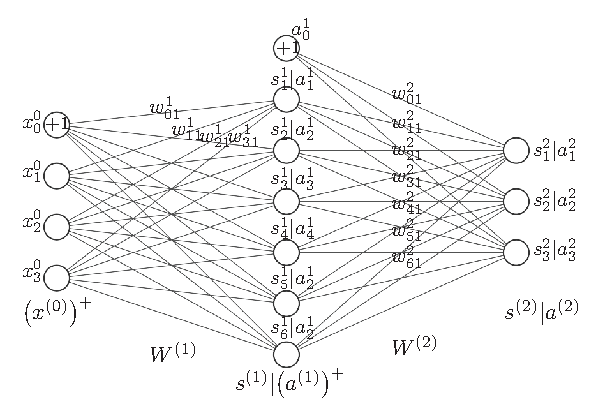
\includegraphics[width=0.72\textwidth]{FC.eps}
  \caption{推导示例神经网络}
  \label{fig:NNFC}
\end{figure}

推导过程中用到大量的变量在此进行解释说明。推导过程中用到自定义的矩阵的一元运算,在此补充。
\begin{table}[!htbp]
%\label{}
\setlength{\tabcolsep}{2.5mm}{
\caption{神经网络参数相关符号}
\begin{tabular}{|l|l|l|}
%\multicolumn{2}{l}{~~~~~~~~~~~~~~~~~~\textbf{神经网络参数}}\\
\hline
\textbf{符号}\hspace{5em} & \textbf{含义}   &\textbf{备注}       \\  \hline
$N_t$ & 训练样本维度      &    $N_t>0$                                                                                                      \\
$N_T$ &  训练样本数量      &  $N_T>0$                                                                                                       \\
$N^{(i)}$ & 第i层神经元个数 & $i\in \{0,1,2,\cdots,H+1\}~~~~i=H+1$表示输出层~~不带Bias\\
$H$ & 隐藏层数       & 包含H个隐藏层                   \\
 K     &  分类类别数       &   $K>1$                                                                                                     \\
 $S_l$ & 损失函数        &$S_l\in \{\text{Mean~~Square ~~Error,Cross~~Entropy~~Loss}\}$                                                               \\ \hline
\end{tabular}}
\end{table}

\begin{table}[!!htbp]
%\label{}
\caption{神经网络推导相关符号}
\setlength{\tabcolsep}{2.5mm}{
\begin{tabular}{|l|l|l|}
%\multicolumn{3}{l}{~~~~~~~~~~~~~~~~~~\textbf{示例推导相关符号}}\\
\hline
\textbf{符号} & \textbf{含义}    & \textbf{备注}       \\  \hline
$\bm{x}$                         & 输入行向量    &一个训练样本特征为一个行向量\\
$\bm{y}$                         & 标签向量        &一个训练样本标签为一个行向量 (ONEHOT)   \\
$\bm{s}$                         & 求和值行向量&每层对应一个行向量       \\
$\bm{a}$                         & 激活值行向量&每层对应一个行向量       \\
$\sigma$                         & 激活函数&$\sigma \in {\text\{sigmoid,tanh,relu,leaky relu,softmax}\}$       \\
$\bm{\cdot}^{(i)}_j$             & i代表网络层次~~~j代表分量&$0\leq i\leq H+1$      \\
\hline
%\multicolumn{2}{l}{~~~~~~~~~~~~~~~~~~}\\
%\multicolumn{2}{l}{~~~~~~~~~~~~~~~~~~\textbf{矩阵化推导相关符号}}\\
\hline
\textbf{符号}\hspace{5em} & \textbf{含义}   &\textbf{备注}       \\  \hline
%$(\cdot)^T$                  & 向量或者矩阵的转置 \\
%$\odot$                         & 按元素相乘  \\
%$\|\cdot\|_p$                         & $L_p$范数     \\
%$\|\cdot\|$                         & $L_2$范数     \\
%$\sum$                         & 连加     \\
%$\prod$                         & 连乘     \\ \hline
$\bm{X}$           & 输入训练样本       & 维度 $N_T\times N_t$~~相当激活值矩阵$A^{(0)}$                                                                        \\
$\bm{X}^+$           & 输入训练样本加偏置列       & 维度 $N_T\times (N_t+1)$~~相当激活值矩阵$\big(A^{(0)}\big)^+$                                                                        \\
$\bm{S}^{(i)}$   & 第 i 层求和值矩阵 & 维度 $N_T\times N^{(i)}$~~$i=1,\cdots,H,H+1$                                                                              \\
$\bm{A}^{(i)}$   & 第 i 层激活值矩阵 & 维度 $N_T\times N^{(i)}$~~$i=0,1,\cdots,H,H+1$                                                                              \\
$\big(\bm{A}^{(i)}\big)^+$   & 第 i 层激活值矩阵加偏置列 & 维度 $N_T\times (N^{(i)}+1)$~~$i=0,1,\cdots,H$                                                                            \\
$\bm{W}^{(i)}$   & 第 i 层权值矩阵  & 维度 $N^{(i-1)}\times N^{(i)}$, $i=1,\cdots,H,H+1$.                                                                                                  \\
$\bm{W}^{(H+1)}$ & 输出层权值矩阵      & 维度 $N^{(N)}\times K$~~标签有 K 个类目                                                                                   \\
$\bm{W}_b^{(i)}$   & 第 i 层权值偏置矩阵  & 维度 $(N^{(i-1)}+1)\times N^{(i)}$, $i=1,\cdots,H,H+1$.                                                                                                  \\
$\bm{W}_b^{(H+1)}$   &输出层权值偏置矩阵  & 维度 $(N^{(N)}+1)\times K$~~标签有 K 个类目                                                                                               \\
$\bm{S}^{(H+1)}$ & 输出层求和值矩阵     & 维度 $N_T\times K $                                                                                                           \\
$\bm{A}^{(H+1)}$ & 输出层激活值矩阵     & 维度 $N_T\times K $                                                                                                      \\
$\bm{Y}$ & 训练数据标签 & 维度 $N_T \times K$ (ONE-HOT)\\
$\bm{\Delta}^{(i)}$ & 反向传播中间变量矩阵 & 维度 $N_T \times N^{(i)}$~~$i=1,\cdots,H,H+1$\\
$\bm{\Delta}^{(H+1)}$ & 输出层反向传播中间变量矩阵 & 维度 $N_T \times K$\\ \hline
\end{tabular}}
\end{table}


\begin{definition}
  ~~~~~~$\bm{x}^+$ 运算符:为向量$\bm{x}$添加$Bias$列,具体在第$0$列添加全$1$。
\end{definition}

\begin{example}
  ~~~~~~~~~~~~$\bm{x} = \left(
 \begin{matrix}
   a & b & c \\
   d & e & f \\
   g & h & i
  \end{matrix}
  \right) $~~~~~~
  $\bm{x}^+ = \left(
\begin{matrix}
   1 & a & b & c \\
   1 & d & e & f \\
   1 & g & h & i
  \end{matrix}
  \right) $
\end{example}

\begin{definition}
  ~~~~~~$\bm{x}^-$ 运算符:为向量$\bm{x}$删去$Bias$列,具体删除第$0$列。
\end{definition}

\begin{example}
~~~~~~~~~~~~$\bm{x} = \left(
 \begin{matrix}
   a & b & c \\
   d & e & f \\
   g & h & i
  \end{matrix}
  \right) $~~~~~~
  $\bm{x}^- = \left(
\begin{matrix}
    b & c \\
    e & f \\
    h & i
  \end{matrix}
  \right) $
\end{example}






\section{神经网络正向传播}
\begin{itemize}
  \item 示例推导:
      \begin{align*}
       & \big(\bm{x}^{(0)}\big)^+\bm{W}^{(1)}=\bm{s}^{(1)},~~~\sigma(\bm{s}^{(1)})=\bm{a}^{(1)}\\
        & \big(\bm{a}^{(1)}\big)^+\bm{W}^{(2)}=\bm{s}^{(2)},~~~\sigma(\bm{s}^{(2)})=\bm{a}^{(2)} \\
        & Loss~~~L=\frac{1}{2}\sum_{k=1}^{3}(\bm{a}^{(2)}_k-\bm{y}_k)^2
      \end{align*}

  \item 矩阵扩展推导形式:
    \begin{align*}
       \big(\bm{A}^{(0)}\big)^+\bm{W}_b^{(1)}=\bm{S}^{(1)}\stackrel{\sigma+b}{\longrightarrow} \big(\bm{A}^{(1)}\big)^+&\Rightarrow \cdots \Rightarrow \cdots \\
      & \Rightarrow \big(\bm{A}^{(H-1)}\big)^+\bm{W}_b^{(H)}=\bm{S}^{(H)} \stackrel{\sigma+b}{\longrightarrow}\big(\bm{A}^{(H)}\big)^+  \\
      & \Rightarrow \big(\bm{A}^{(H)}\big)^+\bm{W}_b^{(H+1)}=\bm{S}^{(H+1)}\stackrel{\sigma}{\longrightarrow} \bm{A}^{(H+1)} \\
      & \Rightarrow ~\mathcal{L}(\bm{A}^{(H+1)},\bm{Y})
    \end{align*}
\end{itemize}
\section{神经网络反向传播\cite{BP}}
\begin{itemize}
  \item 示例推导:
    \begin{enumerate}[(1)]
    \item 输出层权值梯度:
  \begin{align*}
    Loss,~~~L&=\frac{1}{2}\sum_{i=1}^{K}(\bm{a}^{(2)}_i-\bm{y}_i)^2\\
    \frac{\partial L}{\partial \bm{W}^{(2)}_{ik}}&=\frac{\partial}{\partial \bm{W}^{(2)}_{ik}}\frac{1}{2}\sum_{i=1}^{K}(\bm{a}^{(2)}_i-\bm{y}_i)^2\\
    &=\big(\sigma(\bm{S}^{(2)}_k)-\bm{y}_k\big)\sigma(\bm{S}^{(2)}_k)\big(1-\sigma(\bm{S}^{(2)}_k)\big)\frac{\partial \bm{S}^{(2)}_k}{\partial \bm{W}^{(2)}_{ik}}\\
    &=\big(\sigma(\bm{S}^{(2)}_k)-\bm{y}_k\big)\sigma(\bm{S}^{(2)}_k)\big(1-\sigma(\bm{S}^{(2)}_k)\big)\big(\bm{a}^{(1)}_i\big)^+\\
    \text{令,}~~\bm{\delta}^{(2)}_k&=\big(\sigma(\bm{S}^{(2)}_k)-\bm{y}_k\big)\sigma(\bm{S}^{(2)}_k)\big(1-\sigma(\bm{S}^{(2)}_k)\big)\\
    &=\big(\bm{a}^{(2)}_k-\bm{y}_k\big)\bm{a}^{(2)}_k\big(1-\bm{a}^{(2)}_k\big)\\
    \text{则,}\frac{\partial L}{\partial \bm{W}^{(2)}_{ik}}&=\bm{\delta}^{(2)}_k\big(\bm{a}^{(1)}_i\big)^+
  \end{align*}
    \item 隐藏层权值梯度:
\begin{align*}
       \frac{\partial L}{\partial \bm{W}^{(1)}_{ij}}&=\frac{\partial}{\partial \bm{W}^{(1)}_{ij}}\frac{1}{2}\sum_{k\in K}(\bm{a}^{(2)}_k-\bm{y}_k)^2\\
       &=\sum_{k\in K}(\bm{a}^{(2)}_k-\bm{y}_k)\frac{\partial \sigma(\bm{s}^{(2)}_k)}{\partial  \bm{W}^{(1)}_{ij}}\\
       &=\sum_{k\in K}(\bm{a}^{(2)}_k-\bm{y}_k)\sigma(\bm{s}^{(2)}_k)\big(1-\sigma(\bm{s}^{(2)}_k)\frac{\partial \bm{s}^{(2)}_k}{\partial  \bm{W}^{(1)}_{ij}}\\
       &=\sum_{k\in K}(\bm{a}^{(2)}_k-\bm{y}_k)\sigma(\bm{s}^{(2)}_k)\big(1-\sigma(\bm{s}^{(2)}_k)\frac{\partial \bm{s}^{(2)}_k}{\partial  \bm{a}^{(1)}_{j}}\frac{\partial \bm{a}^{(1)}_{j}}{\partial  \bm{W}^{(1)}_{ij}}\\
       &=\sum_{k\in K}(\bm{a}^{(2)}_k-\bm{y}_k)\sigma(\bm{s}^{(2)}_k)\big(1-\sigma(\bm{s}^{(2)}_k)\bm{W}^{(2)}_{jk}\frac{\partial \bm{a}^{(1)}_{j}}{\partial  \bm{W}^{(1)}_{ij}}\\
       &=\frac{\partial \bm{a}^{(1)}_{j}}{\partial  \bm{W}^{(1)}_{ij}}\sum_{k\in K}(\bm{a}^{(2)}_k-\bm{y}_k)\sigma(\bm{s}^{(2)}_k)\big(1-\sigma(\bm{s}^{(2)}_k)\bm{W}^{(2)}_{jk}\\
       &=\bm{a}^{(1)}_j\big(1-\bm{a}^{(1)}_j\big)\frac{\partial \bm{s}^{(1)}_j}{\bm{W}^{(1)}_{ij}}\sum_{k\in K}\bm{\delta}^{(2)}_k\bm{W}^{(2)}_{jk}\\
       &=\bm{a}^{(1)}_j\big(1-\bm{a}^{(1)}_j\big)\big(x^{(0)}_i\big)^+\sum_{k\in K}\bm{\delta}^{(2)}_k\bm{W}^{(2)}_{jk}\\
       \text{令, }~~~ \bm{\delta}^{(1)}_j &= \bm{a}^{(1)}_j(1-\bm{a}^{(1)}_j)\sum_{k \in K} \bm{\delta}^{(2)}_k\bm{W}^{(2)}_{jk}\\
       \text{则,} \frac{\partial L}{\partial \bm{W}^{(1)}_{ij}}&= \bm{\delta}^{(1)}_j \big(\bm{x}_i^{(0)}\big)^+
    \end{align*}
  \end{enumerate}
  \item 矩阵扩展推导形式:
\begin{enumerate}
  \item 输出层权值求导:
  \begin{align*}
  \nabla_{\bm{W}_b^{(H+1)}}\mathcal{L}(\bm{A}^{(H+1)},\bm{Y}) &= \frac{1}{H_T}(\bm{A}^{(H)^+})^T\bm{\Delta}^{(H+1)}~~~~~~\text{(矩阵化)}\\
  \bm{\Delta}^{(H+1)}& = \frac{\partial \mathcal{L}(\bm{A}^{(H+1)}, \bm{Y})}{\partial \bm{A}^{(H+1)}}\circ\sigma'(\bm{S}^{(H+1)})\\
  \text{当输出层使用 Soft}&\text{max+CrossEntropy 时:}\\
  \bm{\Delta}^{(H+1)} &= \bm{A}^{(H+1)} - \bm{Y}
\end{align*}
  \item 隐藏层权值求导:
\begin{align*}
  \nabla_{\bm{W}_b^{(H)}}\mathcal{L}(\bm{A}^{(H+1)},\bm{Y})&= \frac{1}{H_T}\big(\bm{A}^{(H-1)^+}\big)^T\bm{\Delta}^{(H)}\\
                                \text{令:}       \bm{\Delta}^{(H)} &=  \big(\bm{\Delta}^{(H+1)}(\bm{W}^{(H+1)})^T\big)\circ \sigma'^{(H)}(\bm{S}^{(H)})\\
    \text{\textcolor{red}{扩展:~对于第 i 个隐藏层}}&\text{\textcolor{red}{的权值矩阵的梯度为($i=1,2,\cdots,H.$):}}\\
    \nabla_{\bm{W}_b^{(i)}}\mathcal{L}(\bm{A}^{(H+1)},\bm{Y})&= \frac{1}{H_T}\big(\bm{A}^{(i-1)^+}\big)^T\bm{\Delta}^{(i)}\\
                                \text{令:}       \bm{\Delta}^{(i)} &=  \bm{\Delta}^{(i+1)}(\bm{W}^{(i+1)})^T\circ\sigma'^{(i)}(\bm{S}^{(i)})
\end{align*}
\end{enumerate}
\end{itemize}
\section{神经网络张量流}

探究神经网络运算过程中的张量变化能更清楚的了解神经网络的作用规律,表(\ref{tb:tensorflow})展示了神经网络的张量流。

\begin{table}[!h]
\label{tb:tensorflow}
\caption{神经网络张量流}
\setlength{\tabcolsep}{9mm}{
\begin{tabular}{|l|l||l|l|}
\hline
前向传播          & 维度                        & 反向传播                                                 & 维度                                  \\ \hline \hline
$\bm{X}$             & $N_T\times (N_t+1)$       & LOSS                                               & Scalar                           \\ \hline
$\bm{S}^{(1)}$     & $N_T\times N^{(1)}$       & $\bm{\Delta}^{(H+1)}$                                     & $N_T\times K$                       \\ \hline
$(\bm{A}^{(1)})^+$     & $N_T\times (N^{(1)}+1)$     & $\nabla_{\bm{W}^{(H+1)}}\mathcal{L}$   & $(N^{(H)}+1)\times K$           \\ \hline
$\bm{S}^{(2)}$     & $N_T\times N^{(2)}$       & $\bm{\Delta}^{(H)}$                                   & $N_T\times (N^{(H)}+1)$         \\ \hline
$(\bm{A}^{(2)})^+$     & $N_T\times (N^{(2)}+1)$     & $\nabla_{\bm{W}^{(N)}}\mathcal{L}$ & $(N^{(H-1)}+1)\times N^{(H)}$ \\ \hline
$\vdots$       & $\vdots$                   & $\vdots$                                              & $\vdots$                             \\ \hline
$\bm{S}^{(H)}$ & $N_T\times N^{(H)}$   & $\bm{\Delta}^{(i)}$                                       & $N_T\times (N^{(i)}+1)$             \\ \hline
$(\bm{A}^{(H)})^+$ & $N_T\times (N^{(H)}+1)$ & $\nabla_{\bm{W}^{(i)}}\mathcal{L}$     & $(N^{(i-1)}+1)\times N^{(i)}$       \\ \hline
$\bm{S}^{(H+1)}$   & $N_T\times K$             & $\bm{\Delta}^{(1)}$                                       & $N_T\times (N^{(1)}+1)$             \\ \hline
$\bm{A}^{(H+1)}$   & $N_T\times K$             & $\nabla_{\bm{W}^{(1)}}\mathcal{L}$     & $(N_t+1)\times N^{(1)}$             \\ \hline
\multicolumn{2}{|c||}{计算求得损失}              & \multicolumn{2}{c|}{更新权值}                   \\ \hline
\end{tabular}}
\end{table}

\chapter{神经网络优化方法}
在当神经网络一次正反向传播后,得到权值梯度,接下来需要进行优化去更新梯度。优化是指寻找可以让函数最小化或最大化的参数的过程。其中梯度下降是优化算法的核心,Adam优化算法为其变种。


\section{梯度下降优化方法}
\subsection{批量梯度下降优化方法}
批量梯度下降法(Batch Gradient Descent,BGD)是最原始的形式,它是指在每一次迭代时使用所有样本来进行梯度的更新\cite{DBLP:journals/connection/Neelakanta96}。具体步骤是:
\begin{enumerate}
  \item 对目标函数求关于每个权值的偏导:$$\frac{\partial J\left(\bm{\theta}_{0}, \bm{\theta}_{1}\right)}{\partial \bm{\theta}_{j}}=\frac{1}{m} \sum_{i=1}^{m}\left(h_{\bm{\theta}}\left(\bm{x}^{(i)}\right)-\bm{y}^{(i)}\right) \bm{x}_{j}^{(i)}$$

其中 $i=1,2,\cdots,m$ 表示样本数, $j=0,1$ 表示特征数,这里我们使用了偏置项 $x_0^{(i)}=1$ 。
  \item 每次迭代对参数进行更新: $$\bm{\theta}_{j}:=\bm{\theta}_{j}-\alpha \frac{1}{m} \sum_{i=1}^{m}\left(h_{\bm{\theta}}\left(\bm{x}^{(i)}\right)-\bm{y}^{(i)}\right) \bm{x}_{j}^{(i)}$$
\end{enumerate}

\begin{titledbox}{梯度下降优化方法伪码\cite{DBLP:journals/nn/WilsonM03}}
$\begin{array}{l}{\text { repeat }} \\  { \qquad\text { for }j=0,1} \\{\qquad \qquad \begin{array}{l}{\bm{\theta}_{j}:=\bm{\theta}_{j}-\alpha \frac{1}{m} \sum_{i=1}^{m}\left(h_{\bm{\theta}}\left(\bm{x}^{(i)}\right)-\bm{y}^{(i)}\right) \bm{x}_{j}^{(i)}} \end{array}}\end{array}$
\end{titledbox}



\begin{enumerate}
  \item 优点:
\begin{itemize}
  \item 一次迭代是对所有样本进行计算,此时利用矩阵进行操作,实现了并行。
  \item 由全数据集确定的方向能够更好地代表样本总体,从而更准确地朝向极值所在的方向。当目标函数为凸函数时,BGD一定能够得到全局最优。
\end{itemize}
  \item 缺点:
\begin{itemize}
  \item 当样本数目 m 很大时,每迭代一步都需要对所有样本计算,训练过程很慢。
\end{itemize}
\end{enumerate}





\subsection{随机梯度下降优化方法}
随机梯度下降法(Stochastic Gradient Descent,SGD)不同于批量梯度下降,随机梯度下降是每次迭代使用一个样本来对参数进行更新\cite{DBLP:journals/ijon/Amari93}。使得训练速度加快。具体步骤是:

\begin{enumerate}
  \item 对一个样本的目标函数求关于每个权值的偏导:
        $$\frac{\partial J^{(i)}\left(\bm{\theta}_{0}, \bm{\theta}_{1}\right)}{\partial \bm{\theta}_{j}}=\left(h_{\bm{\theta}}\left(\bm{x}^{(i)}\right)-\bm{y}^{(i)}\right) \bm{x}_{j}^{(i)}$$

        其中 $i=1,2,\cdots,m$ 表示样本数, $j=0,1$ 表示特征数,这里我们使用了偏置项 $x_0^{(i)}=1$ 。
  \item 参数更新:
$$\bm{\theta}_{j}:=\bm{\theta}_{j}-\alpha\left(h_{\bm{\theta}}\left(\bm{x}^{(i)}\right)-\bm{y}^{(i)}\right) \bm{x}_{j}^{(i)}$$
\end{enumerate}

\begin{titledbox}{随机梯度下降优化方法伪码}
$\begin{array}{l}{\text { repeat}}\\{\qquad\begin{array}{l}{\text{for}~i=1,\cdots,m}\\ {\qquad\text { for }j=0,1} \\{\qquad\qquad\bm{\theta}_{j}:=\bm{\theta}_{j}-\alpha \left(h_{\bm{\theta}}\left(\bm{x}^{(i)}\right)-\bm{y}^{(i)}\right) \bm{x}_{j}^{(i)}}\end{array}}\end{array}$
\end{titledbox}


\begin{enumerate}
  \item 优点:
\begin{itemize}
  \item 由于不是在全部训练数据上的损失函数,而是在每轮迭代中,随机优化某一条训练数据上的损失函数,这样每一轮参数的更新速度大大加快。
\end{itemize}
  \item 缺点:
\begin{itemize}
  \item 准确度下降。由于即使在目标函数为强凸函数的情况下,SGD仍旧无法做到线性收敛。
  \item 可能会收敛到局部最优,由于单个样本并不能代表全体样本的趋势。
  \item 不易于并行实现。
\end{itemize}
\end{enumerate}




\subsection{小批量梯度下降优化方法}
小批量梯度下降优化方法((Mini-Batch Gradient Descent,MBGD))是对 BGD 以及 SGD 的一个折中办法。其思想是:每次迭代 使用 batch\_size 个样本来对参数进行更新。

这里我们假设 batch\_size=10 ,样本数 m=1000 ,$j=0,1$ 表示特征数。


\begin{titledbox}{小批量梯度下降优化方法伪码}
$\begin{array}{l}{\text { repeat }}\\ {\qquad \begin{array}{l}{\text { for } \mathrm{i}=1,11,21,31, \ldots, 991}\\{ \qquad\text { for }j=0,1}\\ {\qquad\qquad\bm{\theta}_{j}:=\bm{\theta}_{j}-\alpha \frac{1}{10} \sum_{k=i}^{(i+9)}\left(h_{\bm{\theta}}\left(\bm{x}^{(k)}\right)-\bm{y}^{(k)}\right) \bm{x}_{j}^{(k)}} \end{array}}\end{array}$
\end{titledbox}



\begin{enumerate}
  \item 优点:
\begin{itemize}
  \item 通过矩阵运算,每次在一个batch上优化神经网络参数并不会比单个数据慢太多。
  \item 每次使用一个batch可以大大减小收敛所需要的迭代次数,同时可以使收敛到的结果更加接近梯度下降的效果。(比如上例中的30W,设置batch\_size=100时,需要迭代3000次,远小于SGD的30W次)
  \item 可实现并行化。
\end{itemize}
  \item 缺点:
\begin{itemize}
  \item batch\_size的不当选择可能会带来一些问题。

\end{itemize}
\end{enumerate}

\begin{information}
利用小批量优化或者随机优化算法相比批量优化算法能快速收敛,减少训练时间。
\end{information}



\section{Adam优化方法}
Adam算法使用了动量变量 $\bm{v}_t$ \cite{DBLP:journals/nn/Qian99}和RMSProp算法中小批量随机梯度按元素平方的指数加权移动平均变量 $\bm{s}_t$ \cite{DBLP:journals/corr/abs-1708-01911},并在时间步0将它们中每个元素初始化为0\cite{DBLP:journals/corr/KingmaB14}。给定超参数 $0<\beta_1<1$ (默认设为0.9),时间步 $t$ 的动量变量 $\bm{v}_t$ 即小批量随机梯度 $\bm{g}_t$ 的指数加权移动平均:
\begin{equation}\label{E:Adam1}
  \bm{v}_t←\beta_1\bm{v}_{t−1}+(1−\beta_1)\bm{g}_t
\end{equation}

和RMSProp算法中一样,给定超参数 $0\leq \beta_2<1$ (默认设为设为0.999), 将小批量随机梯度按元素平方后的项 $\bm{g}_t\odot \bm{g}_t$ 做指数加权移动平均得到 $\bm{s}_t$ :
\begin{equation}\label{E:Adam2}
  \bm{s}_t←\beta_2\bm{s}_{t−1}+(1−\beta_2)\bm{g}_t\odot \bm{g}_t
\end{equation}


由于我们将 $\bm{v}_0$ 和 $\bm{s}_0$ 中的元素都初始化为0, 在时间步 t 我们得到 $\bm{v}_t=(1−\beta_1)\sum^{t}_{i=1}\beta_1^{t-i}\bm{g}_i$ 。将过去各时间步小批量随机梯度的权值相加,得到 $(1−\beta_1) \sum_{i=1}^t  \beta^{t−i}_1=1−\beta^t_1$  。需要注意的是,当 t 较小时,过去各时间步小批量随机梯度权值之和会较小。例如,当 $\beta_1=0.9$ 时, $\bm{v}_1=0.1\bm{g}_1$ 。为了消除这样的影响,对于任意时间步 t ,我们可以将 $\bm{v}_t$ 再除以 $1−\beta^t_1$ ,从而使过去各时间步小批量随机梯度权值之和为1。这也叫作偏差修正。在Adam算法中,我们对变量 $\bm{v}_t$ 和 $\bm{s}_t$ 均作偏差修正:
\begin{equation}\label{E:Adam3}
  \bm{\hat{v}}_t←\frac{\bm{v}_t}{1−\beta^t_1}
\end{equation}
\begin{equation}\label{E:Adam4}
  \bm{\hat{s}}_t←\frac{\bm{s}_t}{1−\beta^t_2}
\end{equation}



接下来,Adam算法使用以上偏差修正后的变量 $\bm{\hat{v}}_t$和 $\bm{\hat{s}}_t$ ,将模型参数中每个元素的学习率通过按元素运算重新调整:
\begin{equation}\label{E:Adam5}
  \bm{g}^′_t←\frac{\eta\bm{\hat{v}}_t}{\sqrt{\bm{\hat{s}}_t}+\epsilon}
\end{equation}


其中 $\eta$ 是学习率, $\epsilon$ 是为了维持数值稳定性而添加的常数,如 $10^{−8}$ 。和AdaGrad算法、RMSProp算法以及AdaDelta算法一样,目标函数自变量中每个元素都分别拥有自己的学习率。最后,使用 $\bm{g}^′_t$ 迭代自变量:
\begin{equation}\label{E:Adam6}
  x_t←x_{t−1}−\bm{g}^′_t
\end{equation}


\begin{titledbox}{Adam权值更新核心伪码}
$\begin{array}{l}
   \qquad\qquad\bm{v}_t=\beta_1\bm{v}_{t-1}+(1-\beta_1)\bm{g}_t\\
   \qquad\qquad\bm{s}_t = \beta_2\bm{s}_{t-1}+(1-\beta_2)\bm{g}_t\odot \bm{g}_t \\
   \qquad\qquad\bm{\hat{v}}_t=\frac{\bm{v}_t}{1-\beta^t_1}\\
   \qquad\qquad\bm{\hat{s}}_t=\frac{\bm{s}_t}{1-\beta^t_2}\\
   \qquad\qquad\bm{g}'_t=\frac{\eta \bm{\hat{v}}_t}{\sqrt{\bm{\hat{s}}_t}+\epsilon}\\
   \qquad\qquad\bm{x}_t = \bm{x}_{t-1}- \bm{g}'_t\end{array}$
\end{titledbox}


\begin{enumerate}
  \item 优点:
    \begin{itemize}
      \item 直截了当地实现。
        \item 高效的计算。
        \item 所需内存少。
        \item 梯度对角缩放的不变性。
        \item 适合解决含大规模数据和参数的优化问题。
        \item 适用于非稳态(non-stationary)目标。
        \item 适用于解决包含很高噪声或稀疏梯度的问题。
        \item 超参数可以很直观地解释,并且基本上只需极少量的调参。

    \end{itemize}
  \item 缺点:
  \begin{itemize}
    \item 特殊状况下可能不收敛。
    \item 可能错过全局最优解。
  \end{itemize}
\end{enumerate}

\part{框架文档}
\chapter{框架结构}

全连接神经网络模型主要以层次建模图(\ref{fig:FCNNFrame}),在以矩阵数据结构的基础上,为神经网络隐藏层次(求和层以及激活层),输出层以及损失层进行模型建设,之后再对神经网络的初始化方式,前向传播,反向传播,优化算法等进行建模。

\begin{enumerate}
  \item 神经网络层次模型
  \begin{enumerate}
    \item 隐藏层
    \begin{enumerate}
      \item 求和层
      \item 激活层
    \end{enumerate}
    \item 输出层
    \item 损失层
  \end{enumerate}
\end{enumerate}



\begin{figure}[!h]%{5cm}
  \centering
  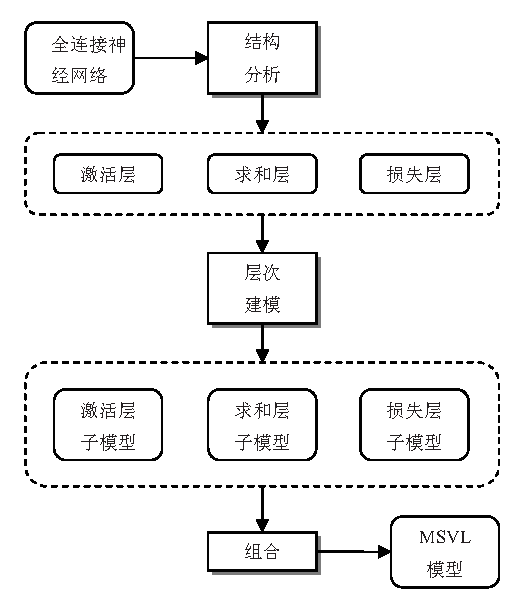
\includegraphics[width=0.35\textwidth]{FCNN.eps}
  \caption{全连接神经网络建模方案}
  \label{fig:FCNNFrame}
\end{figure}



%\begin{lstlisting}[language=C,caption={src/app/app.module.ts}]
%export class Logger {
%  log(msg: any)   { console.log(msg); }
%  error(msg: any) { console.error(msg); }
%  warn(msg: any)  { console.warn(msg); }
%}
%\end{lstlisting}
\chapter{编码说明}

%本章主要对框架中对象结构体各个字段以及主要函数的输入输出进行说明解释,为下一章开发流程中所利用。
\section{对象结构体说明}
\subsection{矩阵结构体}
\begin{lstlisting}[language=C,caption={矩阵结构体}]
struct Mat {
int row,col and     // 矩阵的行数和列数
float **element     // 二维矩阵元素值
};
\end{lstlisting}

\noindent\textbf{注:}
\begin{itemize}
  \item 二维矩阵结构体是本框架最基本的数据结构,一切操作都源于此。
\end{itemize}


\subsection{神经网络单层结构体}
\begin{lstlisting}[language=C,caption={神经网络单层结构体}]
struct FCLayer {
Mat ActiMat and                 // 不带有偏置列的激活值矩阵
Mat ActiMatPlus and             // 带有偏置列的激活值矩阵
Mat SumMat and                  // 求和值矩阵
Mat WeightMat and               // 不带有偏置的权值矩阵
Mat WeightBiasMat and           // 带有偏置的权值矩阵
Mat DeltaMat and                // 反向传播的中间临时矩阵
Mat NablaWbMat and              // 带有偏置的权值梯度矩阵
Mat ActiFunDerivationMat and    // 激活函数导数矩阵
int NeuronNum and               // 神经元个数
int AcitFuncNum                 // 激活函数
};
\end{lstlisting}

\noindent\textbf{注:}
\begin{itemize}
  \item 激活函数整形映射规则见表\ref{T1}。
\end{itemize}


\begin{table}[!ht]
\centering
\caption{激活函数映射规则}
\label{T1}
\setlength{\tabcolsep}{12mm}{
\begin{tabular}{|c|l|}
\hline
\multicolumn{1}{|l|}{整型变量值} & 激活函数          \\ \hline \hline
0                           & no activation \\ \hline
1                           & sigmoid       \\ \hline
2                           & tanh          \\ \hline
3                           & relu          \\ \hline
4                           & leak relu     \\ \hline
5                           & softmax       \\ \hline
\end{tabular}}
\end{table}




\subsection{神经网络结构体}

\begin{lstlisting}[language=C,caption={神经网络结构体}]
struct FCNN {
int CurrentSampleNum and        // 当前神经网络处理的样本数量
int SampleDimensionNum and      // 样本的特征数
int HiddenLayerNum and          // 隐藏层个数
int WeightInitWayNum and        // 权值初始化方式
FCLayer *Layer and              // 神经网络所有层
Mat OnehotMat and               // onehot 编码的标签
int ClassificationNum and       // 神经网络的分类个数
int LossFuncNum                 // 损失函数
};
\end{lstlisting}

\noindent\textbf{注:}
\begin{itemize}
  \item 权值初始化方式映射规则见表\ref{T2}以及损失函数映射规则见表\ref{T3}。
\end{itemize}


\begin{table}[!hb]
\centering
\caption{权值初始化方式映射规则}
\label{T2}
\setlength{\tabcolsep}{12mm}{
\begin{tabular}{|c|l|}
\hline
整型变量值 & 初始化方式     \\ \hline \hline
0     & 全零初始化     \\ \hline
1     & 随机初始化     \\ \hline
2     & xavier初始化 \\ \hline
3     & 凯明初始化     \\ \hline
\end{tabular}}
\end{table}
\begin{table}[!htbp]
\centering
\caption{损失函数映射规则}
\label{T3}
\setlength{\tabcolsep}{12mm}{
\begin{tabular}{|c|l|}
\hline
整型变量值 & 损失函数  \\ \hline \hline
0     & 均方差损失 \\ \hline
1     & 交叉熵损失 \\ \hline
\end{tabular}}
\end{table}

\subsection{数据集结构体}
\begin{lstlisting}[language=C,caption={数据集结构体}]
struct DataSet {
Mat CompleteFeatureDataSet and      // 全体特征数据
Mat CompleteLabelDataSet and        // 全体数据的标签
Mat CompleteTrainFeature and        // 训练特征数据
Mat CompleteTrainLabel and          // 训练数据标签(非独热编码)
Mat *BatchTrainFeature and          // 批量训练特征数据(三维)
Mat *BatchTrainLabel and            // 批量训练数据标签(非独热编码)
Mat *BatchTrainLabelOneHot and      // 批量训练数据标签(独热编码)
Mat TestFeature and                 // 测试特征数据
Mat TestLabel and                   // 测试数据标签(非独热编码)
Mat TestLabelOneHot and             // 测试数据标签(独热编码)
int CompleteSampleNum and           // 全体数据集个数
int TrainSampleNum and              // 训练数据个数
int TestSampleNum and               // 测试数据个数
int SampleDimensionNum and          // 数据样本特征数
int ClassificationNum and           // 分类个数
int BatchSize and                   // 批量数据块大小
int BatchNum and                    // 批量数据块数
int remainder                       // 最后一批数据块大小(看能否整除)
};
\end{lstlisting}

\noindent\textbf{注:}
\begin{itemize}
  \item 余数机制是为了保证神经网络的小批量优化训练数据完整性。
\end{itemize}


\subsection{用户自定义参数结构体}
\begin{lstlisting}[language=C,caption={用户自定义结构体}]
struct Custom {
int CompleteSampleNum and       // 全体数据集个数
int TrainSampleNum and          // 训练数据个数
int TestSampleNum and           // 测试数据个数
int SampleDimensionNum and      // 数据样本特征数
int HiddenLayerNum and          // 神经网络隐藏层个数
int WeightInitWayNum and        // 神经网络初始化方式
float *XValArray and            // 全体特征数据数组
float *YValArray and            // 全体标签数据数组
int *NeuronNumArray and         // 神经网络各层神经元个数
int *ActiFuncNumArray and       // 神经网络各层激活函数
int ClassificationNum and       // 神经网络分类数
int LossFuncNum and             // 损失函数
int BatchSize                   // 批量优化算法块大小
};
\end{lstlisting}


\subsection{Adam优化参数结构体}
\begin{lstlisting}[language=C,caption={Adam优化参数结构体}]
typedef struct {
	float beta1;
	float beta2;
	float eta;
	float epsilon;
	int time;
	Mat *v;
	Mat *hat_v;
	Mat *s;
	Mat *hat_s;
	Mat *hat_g;
}AdamPara;
\end{lstlisting}

\section{基础函数说明}
\subsection{辅助函数}
\begin{table}[!h]
\centering
\caption{辅助函数}
\setlength{\tabcolsep}{4mm}{
\begin{tabular}{|l|l|l|l|l|}
\hline
函数名      & \multicolumn{2}{l|}{输入类型}  & 输出类型   & 功能           \\ \hline \hline
absolute & \multicolumn{2}{c|}{float} & float  & 浮点数绝对值       \\ \hline
min      & float        & float       & float  & 两浮点数较小的一个    \\ \hline
equal    & float        & float       & int    & 判定两浮点数是否相等   \\ \hline
F2S      & float        & char *      & char * & 实现浮点数向字符串的转换 \\ \hline
\end{tabular}}
\end{table}

\begin{information}
\textcolor{red}{由于MSVL编译器对浮点型数据标准输出会出现错误,而能正确标准输出字符串。}所以其中转换函数F2S是解决MSVL编译器对浮点型数据的标准输出问题的一种方案。
\end{information}



\subsection{二维矩阵操作函数}
% Please add the following required packages to your document preamble:
\begin{table}[!h]
\centering
\caption{二维矩阵操作函数}
\setlength{\tabcolsep}{2.5mm}{
\begin{tabular}{|l|l|l|l|l|l|l|}
\hline
编号 & 函数名          & \multicolumn{3}{c|}{输入类型}                                 & 输出类型  & 功能             \\ \hline \hline
1  & MatCreate    & Mat *                      & int           & int          & Mat * & 创建固定行数列数的矩阵空间  \\ \hline
2  & MatDelete    & \multicolumn{3}{c|}{Mat *}                                & NULL  & 删除目标矩阵的空间      \\ \hline
3  & MatSetVal    & \multicolumn{1}{l|}{Mat *} & \multicolumn{2}{l|}{float *} & Mat * & 将数组元素赋值给矩阵     \\ \hline
4  & MatShape     & \multicolumn{3}{c|}{const Mat *}                          & NULL  & 标准输出目标矩阵的行数列数  \\ \hline
5  & MatDump      & \multicolumn{3}{c|}{const Mat *}                          & NULL  & 标椎输出目标矩阵       \\ \hline
6  & MatZeros     & \multicolumn{3}{c|}{Mat *}                                & Mat * & 目标矩阵赋值为全0阵     \\ \hline
7  & MatOnes      & \multicolumn{3}{c|}{Mat *}                                & Mat * & 目标矩阵赋值为全1阵     \\ \hline
8  & MatEye       & \multicolumn{3}{c|}{Mat *}                                & Mat * & 目标矩阵赋值为对角1阵    \\ \hline
9  & MatAdd       & \multicolumn{1}{l|}{Mat *} & Mat *         & Mat *        & Mat * & 前两矩阵相加赋值给末矩阵    \\ \hline
10 & MatSub       & \multicolumn{1}{l|}{Mat *} & Mat *         & Mat *        & Mat * & 前两矩阵相减赋值给末矩阵    \\ \hline
11 & MatMul       & \multicolumn{1}{l|}{Mat *} & Mat *         & Mat *        & Mat * & 前两矩阵相乘赋值给末矩阵    \\ \hline
12 & MatMul2      & \multicolumn{1}{l|}{Mat *} & Mat *         & Mat *        & Mat * & 矩阵相乘赋值给末矩阵(稀疏优化)  \\ \hline
13 & MatProduct   & \multicolumn{1}{l|}{Mat *} & Mat *         & Mat *        & Mat * & 前两矩阵哈曼积赋值给末矩阵   \\ \hline
14 & MatDiv       & \multicolumn{1}{l|}{Mat *} & Mat *         & Mat *        & Mat * & 前两矩阵相除赋值给末矩阵    \\ \hline
15 & MatNumMul    & \multicolumn{1}{l|}{int}   & Mat *         & Mat *        & Mat * & 数乘矩阵赋值给末矩阵     \\ \hline
16 & MatNumAdd    & \multicolumn{1}{l|}{Mat *} & Mat *         & Mat *        & Mat * & 数加矩阵赋值给末矩阵     \\ \hline
17 & MatTrans     & \multicolumn{2}{c|}{Mat *}                 & Mat *        & Mat * & 矩阵转置赋值给末矩阵     \\ \hline
18 & MatRowSum    & \multicolumn{2}{c|}{Mat *}                 & Mat *        & Mat * & 矩阵每一行相加赋值给末矩阵  \\ \hline
19 & MatRowMax    & \multicolumn{2}{c|}{Mat *}                 & Mat *        & Mat * & 矩阵每一行最大值赋值给末矩阵 \\ \hline
20 & MatSquare    & \multicolumn{2}{c|}{Mat *}                 & Mat *        & Mat * & 矩阵平方赋值给末矩阵     \\ \hline
21 & MatSqrt      & \multicolumn{2}{c|}{Mat *}                 & Mat *        & Mat * & 矩阵开根号赋值给末矩阵    \\ \hline
22 & MatExp       & \multicolumn{2}{c|}{Mat *}                 & Mat *        & Mat * & 矩阵自然底数幂赋值给末矩阵  \\ \hline
23 & MatVectorSub & \multicolumn{1}{l|}{Mat *} & Mat *         & Mat *        & Mat * & 矩阵行减向量赋值给末矩阵   \\ \hline
24 & MatVectorDiv & \multicolumn{1}{l|}{Mat *} & Mat *         & Mat *        & Mat * & 矩阵行除向量赋值给末矩阵   \\ \hline
25 & MatCopy      & \multicolumn{2}{c|}{Mat *}                 & Mat *        & Mat * & 矩阵拷贝赋值给末矩阵     \\ \hline
26 & MatPlusCol   & \multicolumn{3}{c|}{Mat *}                 & Mat * & 矩阵一列扩展赋值给末矩阵   \\ \hline
27   & MatPlusRow   & \multicolumn{3}{c|}{Mat *}               & Mat * & 矩阵一行扩展赋值给末矩阵   \\ \hline
\end{tabular}}
\end{table}

\noindent\textbf{注:}
\begin{itemize}
  \item 函数${12}$ MatMul2 矩阵乘法是对函数$11$ MatMul 矩阵乘法关于稀疏矩阵的优化\cite{DBLP:conf/aiccsa/EmadHM05}。
  \item  函数${13}$ MatProduct 矩阵哈曼积是同维矩阵对应元素相乘,区别于矩阵乘法。
  \item 函数$20,21,22$ MatSquare, MatSqrt, MatExp 均是对矩阵中的每一个元素进行一元运算。
  \item 函数${23}$ MatVectorSub 矩阵向量减得运算规则是:$$\bm{D}_{m\times n},~ \bm{A}_{m\times n},~ \bm{B}_{m\times 1}: ~~~~~~\bm{D}_{ij} = \bm{A}_{ij} - \bm{B}_{i1}$$
  \item 函数${26}$ MatPlusCol 矩阵列扩展规则是目标矩阵的最左列扩展一列并全部赋值为1;函数${27}$ MatPlusRow 类似。
\end{itemize}

\begin{information}
函数$12$ MatMul2 矩阵乘法关于稀疏矩阵的优化,相比函数$11$ MatMul 此举可将大大减少神经网络的训练时间。代码详见例(\ref{ex:mul})。
\end{information}

\begin{example}\label{ex:mul}
    矩阵乘法代码:
  \begin{lstlisting}[language=C,caption={函数 11 MatMul}]
function MatMul ( Mat *src1,Mat *src2,Mat *dst,Mat* RValue )
 {
     frame(MatMul_row,MatMul_col,MatMul_i,MatMul_temp,return) and (
     int return<==0 and skip;
     int MatMul_row,MatMul_col and skip;
     int MatMul_i and skip;
     float MatMul_temp and skip;
     MatMul_row:=0;

     while( (MatMul_row<dst->row) )
     {
         MatMul_col:=0;

         while( (MatMul_col<dst->col) )
         {
             MatMul_temp:=0.0;
             MatMul_i:=0;

             while( (MatMul_i<src1->col) )
             {
                 MatMul_temp:=MatMul_temp+(src1->element[MatMul_row])[MatMul_i]*(src2->element[MatMul_i])[MatMul_col];
                 MatMul_i:=MatMul_i+1
             };
             (dst->element[MatMul_row])[MatMul_col]:=MatMul_temp;
             MatMul_col:=MatMul_col+1
         };
         MatMul_row:=MatMul_row+1
     };
     return<==1 and RValue:=dst;
     skip
     )
     };
\end{lstlisting}

\begin{lstlisting}[language=C,caption={函数 12 MatMul2}]
function MatMul2 ( Mat *src1,Mat *src2,Mat *dst,Mat* RValue )
 {
     frame(MatMul2_row,MatMul2_col,MatMul2_i,MatMul2_1_temp$_1,return) and (
     int return<==0 and skip;
     int MatMul2_row,MatMul2_col and skip;
     int MatMul2_i and skip;
     MatZeros(dst,RValue);
     MatMul2_row:=0;

     while( (MatMul2_row<src1->row) )
     {
         MatMul2_col:=0;

         while( (MatMul2_col<src1->col) )
         {
             int MatMul2_1_temp$_1 and skip;
             MatMul2_1_temp$_1:=equal((src1->element[MatMul2_row])[MatMul2_col],0,RValue);
             if(MatMul2_1_temp$_1=0) then               // 判定0因子
             {
                 MatMul2_i:=0;
                 while( (MatMul2_i<src2->col) )
                 {
                     (dst->element[MatMul2_row])[MatMul2_i]:=(dst->element[MatMul2_row])[MatMul2_i]+(src1->element[MatMul2_row])[MatMul2_col]*(src2->element[MatMul2_col])[MatMul2_i];          // 改写二维数组指针为两个一维
                     MatMul2_i:=MatMul2_i+1
                 }
             }
             else
             {
                  skip
             };
             MatMul2_col:=MatMul2_col+1
         };
         MatMul2_row:=MatMul2_row+1
     };
     return<==1 and RValue:=dst;
     skip
     )
     };
\end{lstlisting}

函数$12$ {\setsansfont{Myriad Pro} MatMul2} 相比函数$11$ {\setsansfont{Myriad Pro} MatMul} 对稀疏矩阵优化的核心在于判定零因子,每判定一个零因子将会减少第二个矩阵的列次乘操作,稀疏矩阵的零因子多,因此能提高矩阵乘法的效率。  \hfill$\square$
\end{example}


\begin{information}
\textcolor{red}{MSVL 编译器不支持二维数组指针,将其改写为两个一维。}
\end{information}


\subsection{激活函数相关函数}
\begin{table}[!h]
\centering
\caption{激活函数相关函数}
\setlength{\tabcolsep}{2.5mm}{
\begin{tabular}{|l|l|c|l|l|l|l|}
\hline
编号 & 函数名                    & \multicolumn{3}{c|}{输入类型}              & 输出类型  & 功能              \\ \hline \hline
1  & sigmoid  (公式\ref{E11})              & \multicolumn{3}{c|}{float}             & float & sigmoid激活       \\ \hline
2  & tanh        (公式\ref{E21})           & \multicolumn{3}{c|}{float}             & float & tanh激活          \\ \hline
3  & relu      (公式\ref{E31})             & \multicolumn{3}{c|}{float}             & float & relu激活          \\ \hline
4  & leakyRelu  (公式\ref{E41})            & \multicolumn{2}{l|}{float} & float     & float & leakyRelu激活     \\ \hline
5  & MatSoftmax   (公式\ref{E51})          & \multicolumn{3}{c|}{Mat *}             & Mat * & Softmax激活       \\ \hline
6  & MatNoneActi            & \multicolumn{3}{c|}{Mat *}             & Mat * & 不激活             \\ \hline
7  & MatSigmoid             & \multicolumn{3}{c|}{Mat *}             & Mat * & sigmoid激活矩阵     \\ \hline
8  & MatTanh                & \multicolumn{3}{c|}{Mat *}             & Mat * & tanh激活矩阵        \\ \hline
9  & MatRelu                & \multicolumn{3}{c|}{Mat *}             & Mat * & relu激活矩阵        \\ \hline
10 & MatLeakyRelu           & \multicolumn{3}{c|}{Mat *}             & Mat * & leakyRelu激活矩阵   \\ \hline
11 & MatDerivationSoftmax (公式\ref{E52})  & \multicolumn{3}{c|}{Mat *}             & Mat * & Softmax矩阵求导函数   \\ \hline
12 & MatDerivationNoneActi  & \multicolumn{3}{c|}{Mat *}             & Mat * & 不激活矩阵求导函数       \\ \hline
13 & MatDerivationSigmoid (公式\ref{E12})  & \multicolumn{3}{c|}{Mat *}             & Mat * & sigmoid矩阵求导函数   \\ \hline
14 & MatDerivationTanh  (公式\ref{E22})    & \multicolumn{3}{c|}{Mat *}             & Mat * & tanh矩阵求导函数      \\ \hline
15 & MatDerivationRelu  (公式\ref{E32})    & \multicolumn{3}{c|}{Mat *}             & Mat * & relu矩阵求导函数      \\ \hline
16 & MatDerivationLeakyRelu(公式\ref{E42}) & \multicolumn{3}{c|}{Mat *}             & Mat * & leakyrelu矩阵求导函数 \\ \hline
\end{tabular}}
\end{table}

\noindent\textbf{注:}
\begin{itemize}
  \item 函数$2$ tanh 是利用C语言 math 库中,未重写。
  \item  函数$6$ MatNoneActi 未激活矩阵函数是为了统一规范编写激活函数。
\end{itemize}

\begin{information}
MSVL 编译器可以外部调用C语言的函数库里的函数,将相关函数声明到 MC8.0 项目资源文件 external.c 里适当位置上即可。
\end{information}

\begin{example}
{\setsansfont{Myriad Pro}softmax}及其导函数代码:
  \begin{lstlisting}[language=C,caption={函数 5 MatSoftmax}]
function MatSoftmax ( Mat *src,Mat *dst,Mat* RValue )
 {
     frame(MatSoftmax_tempV,return) and (
     int return<==0 and skip;
     Mat MatSoftmax_tempV and skip;
     MatCreate(&MatSoftmax_tempV,src->row,1,RValue);    //存临时的最大行值以及求和行值向量
     MatRowMax(src,&MatSoftmax_tempV,RValue);           //求最大行值向量
     MatVectorSub(src,&MatSoftmax_tempV,dst,RValue);    //矩阵向量相减
     MatExp(dst,dst,RValue);                            //矩阵求对数
     MatRowSum(dst,&MatSoftmax_tempV,RValue);           //求行求和向量
     MatVectorDiv(dst,&MatSoftmax_tempV,dst,RValue);    //矩阵向量相除
     MatDelete(&MatSoftmax_tempV);
     return<==1 and RValue:=dst;
     skip
     )
     };
\end{lstlisting}

\begin{lstlisting}[language=C,caption={函数 11 MatDerivationSoftmax}]
function MatDerivationSoftmax ( Mat *src,Mat *dst,Mat* RValue )
 {
     frame(MatDerivationSoftmax_row,MatDerivationSoftmax_col,MatDerivationSoftmax_i,return) and (
     int return<==0 and skip;
     int MatDerivationSoftmax_row,MatDerivationSoftmax_col,MatDerivationSoftmax_i and skip;
     MatSoftmax(src,src,RValue);                // 先用 softmax 激活, 在根据公式判断选择。
     MatZeros(dst,RValue);
     MatDerivationSoftmax_row:=0;

     while( (MatDerivationSoftmax_row<src->row) )
     {
         MatDerivationSoftmax_col:=0;

         while( (MatDerivationSoftmax_col<src->col) )
         {
             MatDerivationSoftmax_i:=0;

             while( (MatDerivationSoftmax_i<src->col) )
             {
                 if(MatDerivationSoftmax_i=MatDerivationSoftmax_col) then       // 选择一
                 {
                     (dst->element[MatDerivationSoftmax_row])[MatDerivationSoftmax_col]:=(dst->element[MatDerivationSoftmax_row])[MatDerivationSoftmax_col]+(src->element[MatDerivationSoftmax_row])[MatDerivationSoftmax_i]*(1-(src->element[MatDerivationSoftmax_row])[MatDerivationSoftmax_col])
                 }
                 else                                                           // 选择二
                 {
                     (dst->element[MatDerivationSoftmax_row])[MatDerivationSoftmax_col]:=(dst->element[MatDerivationSoftmax_row])[MatDerivationSoftmax_col]+-(src->element[MatDerivationSoftmax_row])[MatDerivationSoftmax_i]*(src->element[MatDerivationSoftmax_row])[MatDerivationSoftmax_col]
                 };
                 MatDerivationSoftmax_i:=MatDerivationSoftmax_i+1
             };
             MatDerivationSoftmax_col:=MatDerivationSoftmax_col+1
         };
         MatDerivationSoftmax_row:=MatDerivationSoftmax_row+1
     };
     return<==1 and RValue:=dst;
     skip
     )
     };
\end{lstlisting} \hfill$\square$
\end{example}

\subsection{损失函数相关函数}
\begin{table}[!h]
\centering
\caption{损失函数相关函数}
\setlength{\tabcolsep}{2mm}{
\begin{tabular}{|l|l|c|c|c|l|l|}
\hline
编号 & 函数名                    & \multicolumn{3}{c|}{输入类型}            & 输出类型  & 功能             \\ \hline \hline
1  & OneHot                 & Mat *   & int          & Mat *       & Mat * & 进行ONEHOT编码     \\ \hline
2  & MSE(公式\ref{2.2.1.1})                  & Mat *   & \multicolumn{2}{c|}{Mat *} & float & 得到两矩阵的均方误差     \\ \hline
3  & CrossEntropy(公式\ref{2.2.1.3})            & Mat *   & \multicolumn{2}{c|}{Mat *} & float & 得到两矩阵的交叉熵损失    \\ \hline
4  & MSEDerivative(公式\ref{2.2.1.2})           & Mat *   & Mat *        & Mat         & Mat * & 得到均方误差对权值的导函数  \\ \hline
5  & CrossEntropyDerivative(公式\ref{2.2.1.4})  & Mat *   & Mat *        & Mat         & Mat * & 得到交叉熵损失对权值的导函数 \\ \hline
\end{tabular}}
\end{table}

\noindent\textbf{注:}
\begin{itemize}
  \item 函数$1$ OneHot 将参数一(必须是从零开始连续地标签数字向量),按照第二个参数分类数 K,进行ONEHOT编码,形成目标矩阵\cite{DBLP:journals/ivc/RodriguezBGE18}。
\end{itemize}


\begin{example}
交叉熵及其导函数代码:
\begin{lstlisting}[language=C,caption={函数 3 CrossEntropy}]
function CrossEntropy ( Mat *src,Mat *dst,float RValue )
 {
     frame(CrossEntropy_row,CrossEntropy_col,CrossEntropy_loss,return) and (
     int return<==0 and skip;
     int CrossEntropy_row,CrossEntropy_col and skip;
     float CrossEntropy_loss<==0.0 and skip;
     CrossEntropy_row:=0;

     while( (CrossEntropy_row<src->row) )
     {
         CrossEntropy_col:=0;

         while( (CrossEntropy_col<src->col) )
         {
             CrossEntropy_loss:=CrossEntropy_loss+(float)(-1*(dst->element[CrossEntropy_row])[CrossEntropy_col]*log((src->element[CrossEntropy_row])[CrossEntropy_col]));           //	依照公式求总  之后再平均
             CrossEntropy_col:=CrossEntropy_col+1

         };
         CrossEntropy_row:=CrossEntropy_row+1

     };
     CrossEntropy_loss:=CrossEntropy_loss/ (src->row);          // 平均
     return<==1 and RValue:=CrossEntropy_loss;
     skip
     )
     };
\end{lstlisting}

\begin{lstlisting}[language=C,caption={函数 5 CrossEntropyDerivative}]
 function CrossEntropyDerivative ( Mat *ActiMat,Mat *DerivativeActiMat,Mat One_hotMat,Mat* RValue )
 {
     frame(CrossEntropyDerivative_row,CrossEntropyDerivative_col,CrossEntropyDerivative_1_2_temp$_1,return) and (
     int return<==0 and skip;
     int CrossEntropyDerivative_row,CrossEntropyDerivative_col and skip;
     CrossEntropyDerivative_row:=0;

     while( (CrossEntropyDerivative_row<ActiMat->row) )
     {
         CrossEntropyDerivative_col:=0;

         while( (CrossEntropyDerivative_col<ActiMat->col) )
         {
             int CrossEntropyDerivative_1_2_temp$_1 and skip;
             CrossEntropyDerivative_1_2_temp$_1:=equal((ActiMat->element[CrossEntropyDerivative_row])[CrossEntropyDerivative_col],0.0,RValue);
             if(CrossEntropyDerivative_1_2_temp$_1=1) then      // 当除数为零时  为防止除零报错 直接给被除数乘无限大
             {
                 (DerivativeActiMat->element[CrossEntropyDerivative_row])[CrossEntropyDerivative_col]:=-(One_hotMat.element[CrossEntropyDerivative_row])[CrossEntropyDerivative_col]*10000000000

             }
             else       // 正常除
             {
                 (DerivativeActiMat->element[CrossEntropyDerivative_row])[CrossEntropyDerivative_col]:=-(One_hotMat.element[CrossEntropyDerivative_row])[CrossEntropyDerivative_col]/ (ActiMat->element[CrossEntropyDerivative_row])[CrossEntropyDerivative_col]
             };
             CrossEntropyDerivative_col:=CrossEntropyDerivative_col+1

         };
         CrossEntropyDerivative_row:=CrossEntropyDerivative_row+1

     };
     return<==1 and RValue:=DerivativeActiMat;
     skip
     )
     };
\end{lstlisting} \hfill$\square$
\end{example}



\subsection{权值初始化函数}
\begin{table}[!h]
\centering
\caption{激活函数相关函数}
\setlength{\tabcolsep}{2.5mm}{
\begin{tabular}{|l|l|c|l|l|l|l|}
\hline
编号 & 函数名                        & \multicolumn{3}{c|}{输入类型}               & 输出类型  & 功能           \\ \hline \hline
1  & gaussrand\_NORMAL          & \multicolumn{3}{c|}{None}               & float & 随机生成标椎正态分布数据   \\ \hline
2  & gaussrand                  & float      & \multicolumn{2}{l|}{float} & float & 随机生成指定正态分布数据 \\ \hline
3  & MatInitZero                & \multicolumn{3}{c|}{Mat *}              & Mat * & 全零初始化        \\ \hline
4  & MatInitRandomNormalization & \multicolumn{3}{c|}{Mat *}              & Mat * & 随机初始化       \\ \hline
5  & MatInitXavier(公式\ref{Eq:Xavier})              & \multicolumn{3}{c|}{Mat *}              & Mat * & Xavier初始化    \\ \hline
6  & MatInitHe(公式\ref{Eq:Kai})             & \multicolumn{3}{c|}{Mat *}              & Mat * & 凯明初始化        \\ \hline
\end{tabular}}
\end{table}

\noindent\textbf{注:}
\begin{itemize}
  \item 所有的权值初始化均不包括Bias,Bias初始化成零。
  \item 函数$1$ gaussrand\_NORMAL 生成正态分布数据采用的是 Box-Muller 方法。
  \item 函数$4$ MatInitRandomNormalization 随机初始生成是$~\mu = 0, ~~\sigma = 0.1~$正态分布数据。
\end{itemize}

\begin{example}
{\setsansfont{Myriad Pro}Xavier}初始化以及凯明初始化代码:
\begin{lstlisting}[language=C,caption={函数 5 MatInitXavier}]
function MatInitXavier ( Mat *src,Mat* RValue )
 {
     frame(MatInitXavier_temp$_1,MatInitXavier_row,MatInitXavier_col,return) and (
     int return<==0 and skip;
     int MatInitXavier_temp$_1 and skip;
     MatInitXavier_temp$_1:=time(NULL);
     srand((unsigned int)MatInitXavier_temp$_1) and skip;
     int MatInitXavier_row,MatInitXavier_col and skip;
     MatInitXavier_row:=0;

     while( (MatInitXavier_row<src->row) )
     {
         MatInitXavier_col:=0;

         while( (MatInitXavier_col<src->col) )
         {
             (src->element[MatInitXavier_row])[MatInitXavier_col]:=gaussrand(0.0,0.1,RValue)*(float)sqrt(1.0/ src->row);        // 依照公式  每项生成
             MatInitXavier_col:=MatInitXavier_col+1

         };
         MatInitXavier_row:=MatInitXavier_row+1
     };
     return<==1 and RValue:=src;
     skip
     )
     };
\end{lstlisting}

\begin{lstlisting}[language=C,caption={函数 6 MatInitHe}]
 function MatInitHe ( Mat *src,Mat* RValue )
 {
     frame(MatInitHe_row,MatInitHe_col,return) and (
     int return<==0 and skip;
     srand(19950826) and skip;
     int MatInitHe_row,MatInitHe_col and skip;
     MatInitHe_row:=0;

     while( (MatInitHe_row<src->row) )
     {
         MatInitHe_col:=0;

         while( (MatInitHe_col<src->col) )
         {
             (src->element[MatInitHe_row])[MatInitHe_col]:=gaussrand(0.0,0.9,RValue)*(float)sqrt(2.0/ src->row);        // 依照公式  每项生成
             MatInitHe_col:=MatInitHe_col+1

         };
         MatInitHe_row:=MatInitHe_row+1
     };
     return<==1 and RValue:=src;
     skip
     )
     };
\end{lstlisting} \hfill$\square$
\end{example}




\section{开发流程及其函数说明}

\begin{keypoint}
\noindent\textbf{具体开发流程:}
\begin{enumerate}
  \item 用户自定义参数录入
  \item 数据集构建
  \item 神经网络初始化
  \item 前向传播构建
  \item 反向传播构建
  \item 优化算法构建
  \item 神经网络训练构建
  \item 神经网络测试构建
\end{enumerate}
\end{keypoint}

\subsection{用户自定义参数录入}
\begin{keypoint}
目的是将相关参数及总的数据赋值给用户自定义结构体中(其中注意对数组数据的赋值,传引用即可),再将各个参数分发给各个结构体。
\end{keypoint}

\begin{table}[!h]
\centering
\caption{用户自定义参数录入相关函数}
\setlength{\tabcolsep}{2.5mm}{
\begin{tabular}{|l|l|c|c|c|l|l|}
\hline
编号 & 函数名                & \multicolumn{3}{c|}{输入类型}          & 输出类型 & 功能          \\ \hline \hline
1  & InitCustom         & \multicolumn{3}{c|}{Custom *}      & int  & 初始化Custom参数 \\ \hline
2  & DumpFloatArray     & float*  & \multicolumn{2}{c|}{int} & None & 标椎输出浮点型数组   \\ \hline
3  & DumpIntArray       & int*    & \multicolumn{2}{c|}{int} & None & 标椎输出整型数组    \\ \hline
4  & DumpCustom         & \multicolumn{3}{c|}{Custom}        & int  & 标椎输出Custom  \\ \hline
5  & LoadParaFromCustom & Custom  & DataSet *     & FCNN *   & None & 传参到具体结构体中   \\ \hline
\end{tabular}}
\end{table}
\noindent\textbf{注:}
\begin{itemize}
  \item 用户自定义参数的录入,包括整体数据以数组的形式录入。
  \item 四个数组形式的自定义参数单独录入,不再录入函数中录入。
\end{itemize}

\begin{example}
基本参数录入函数代码:
\begin{lstlisting}[language=C,caption={函数 5 LoadParaFromCustom}]
function LoadParaFromCustom ( Custom userDefine,DataSet *dataSet,FCNN *fcnn )
 {
     // Custom ==>> DataSet
     dataSet->BatchSize:=userDefine.BatchSize;
     dataSet->CompleteSampleNum:=userDefine.CompleteSampleNum;
     dataSet->SampleDimensionNum:=userDefine.SampleDimensionNum;
     dataSet->TrainSampleNum:=userDefine.TrainSampleNum;
     dataSet->TestSampleNum:=userDefine.TestSampleNum;
     dataSet->ClassificationNum:=userDefine.ClassificationNum;

     // Custom ==>> FCNN
     fcnn->CurrentSampleNum:=userDefine.BatchSize;              // 代表当前神经网络前向传播时的数据样本的个数
     fcnn->SampleDimensionNum:=userDefine.SampleDimensionNum;
     fcnn->HiddenLayerNum:=userDefine.HiddenLayerNum;
     fcnn->WeightInitWayNum:=userDefine.WeightInitWayNum;
     fcnn->ClassificationNum:=userDefine.ClassificationNum;
     fcnn->LossFuncNum:=userDefine.LossFuncNum
 };
\end{lstlisting}
函数 5 {\setsansfont{Myriad Pro}LoadParaFromCustom} 不包括数组形式的数据录入,以及为创建空间的相关参数的录入。\hfill$\square$
\end{example}

\begin{information}
数组数据的录入,可直接在主函数下传引用即可。
\end{information}

\subsection{数据集构建}

\begin{keypoint}
根据用户输入的数据相关参数将训练测试数据集构建完成。构建路线:
\begin{enumerate}
  \item 根据训练集数据量以及 $\text{Batch\_Size}$ 大小计算并导入相关参数。
  \item 根据整体数据集的各个参数,开辟所需的全部空间。
  \item 录入数据集。
  \begin{enumerate}
  \item 将整体数据集数组根据训练测试集数目划分成两个数组,包括训练特征数组和训练标签数组,测试特征数组和测试标签数组。
  \item 再将训练特征数组和训练标签数组划分成若干个块大小的块训练特征数组和块训练标签数组。
  \item 最后将数据喂入到相应的矩阵结构体当中。
  \end{enumerate}

\end{enumerate}
\end{keypoint}


\begin{table}[!h]
\centering
\caption{数据集构建相关函数}
\setlength{\tabcolsep}{2.5mm}{
\begin{tabular}{|l|l|c|c|l|l|l|}
\hline
编号 & 函数名                         & \multicolumn{3}{c|}{输入类型}                      & 输出类型 & 功能           \\ \hline \hline
1  & InitDataSet                 & \multicolumn{3}{c|}{DataSet *}                 & int  & 初始化DataSet参数 \\ \hline
2  & CalculateAndLoadDataSetPara & \multicolumn{3}{c|}{DataSet *}                 & None & 计算相关参数并录入    \\ \hline
3  & CreateDataSetSpace          & \multicolumn{3}{c|}{DataSet *}                 & None & 创建数据集所需空间    \\ \hline
4  & DataLoading                 & Custom        & \multicolumn{2}{c|}{DataSet *} & int  & 录入矩阵形式数据集    \\ \hline
5  & DatasetConstruction         & Custom        & \multicolumn{2}{c|}{DataSet *} & None & 数据及构建主函数     \\ \hline
\end{tabular}}
\end{table}
\noindent\textbf{注:}
\begin{itemize}
  \item 总体数据集分开成为训练集和测试集,暂不分出验证集。
\end{itemize}

\begin{example}
数据及构建函数代码:
\begin{lstlisting}[language=C,caption={函数 5 DatasetConstruction}]
  function DatasetConstruction ( Custom userDefine,DataSet *dataSet )
 {
     CalculateAndLoadDataSetPara(dataSet);      // 步骤1
     CreateDataSetSpace(dataSet);               // 步骤2
     DataLoading(userDefine,dataSet,RValue)     // 步骤3
 };
\end{lstlisting}~\hfill$\square$
\end{example}








\subsection{神经网络初始化}
\begin{keypoint}
\paragraph{神经网络初始化}
\begin{enumerate}
  \item 开辟神经网络所需空间并导入每层相关参数\textcolor{red}{(注意创建顺序不要变化,1.c 与1.d 可以互换)}
  \begin{enumerate}
    \item 创建神经网络层空间
    \begin{enumerate}
      \item FCLayer
    \end{enumerate}
        \item 导入每层参数
    \begin{enumerate}
      \item AcitFuncNum
      \item NeuronNum
    \end{enumerate}
    \item 创建神经网络运算空间
    \begin{enumerate}
      \item ActiMat
      \item ActiMatPlus
      \item SumMat
      \item ActiFunDerivationMat
      \item DeltaMat
      \item OnehotMat(FCNN)
    \end{enumerate}
    \item 创建神经网络参数空间\textcolor{red}{(参数空间的大小不随输入神经网络样本大小而改变)}
    \begin{enumerate}
      \item WeightMat
      \item WeightBiasMat
      \item NablaWbMat
    \end{enumerate}
  \end{enumerate}
  \item 进行权值初始化
  \begin{enumerate}
    \item WeightMat
    \item WeightBiasMat
  \end{enumerate}
\end{enumerate}
\end{keypoint}


\begin{table}[!h]
\centering
\caption{创建空间及录入相关函数}
\setlength{\tabcolsep}{0.8mm}{
\begin{tabular}{|l|l|c|c|l|l|l|}
\hline
编号 & 函数名                                & \multicolumn{3}{c|}{输入类型}                  & 输出类型      & 功能               \\ \hline \hline
1  & InitFCNN                           & \multicolumn{3}{c|}{FCNN *}                & int       & 初始化FCNN参数        \\ \hline
2  & InitFCLayer                        & \multicolumn{3}{c|}{FCNN *}                & int       & 初始化FCNNLayer参数   \\ \hline
3  & SpaceCreateFCLayer                 & \multicolumn{3}{c|}{FCNN *}                & FCLayer * & 创建FCLayer结构体所需空间 \\ \hline
4  & SpaceCreateActi                    & \multicolumn{3}{c|}{FCNN *}                & None      & 创建激活值矩阵所需空间      \\ \hline
5  & SpaceDeleteActi                    & \multicolumn{3}{c|}{FCNN *}                & None      & 删除激活值矩阵空间        \\ \hline
6  & SpaceCreateActiPlus                & \multicolumn{3}{c|}{FCNN *}                & None      & 创建激活值Plus矩阵所需空间  \\ \hline
7  & SpaceDeleteActiPlus                & \multicolumn{3}{c|}{FCNN *}                & None      & 删除激活值Plus矩阵空间    \\ \hline
8  & SpaceCreateSum                     & \multicolumn{3}{c|}{FCNN *}                & None      & 创建求和值矩阵所需空间      \\ \hline
9  & SpaceDeleteSum                     & \multicolumn{3}{c|}{FCNN *}                & None      & 删除求和值矩阵空间        \\ \hline
10 & SpaceCreateActiFunDerivation       & \multicolumn{3}{c|}{FCNN *}                & None      & 创建激活导函数矩阵所需空间    \\ \hline
11 & SpaceDeleteActiFunDerivation       & \multicolumn{3}{c|}{FCNN *}                & None      & 删除激活导函数矩阵空间      \\ \hline
12 & SpaceCreateDelta                   & \multicolumn{3}{c|}{FCNN *}                & None      & 创建反向中间变量矩阵所需空间 \\ \hline
13 & SpaceDeleteDelta                   & \multicolumn{3}{c|}{FCNN *}                & None      & 删除反向中间变量矩阵空间   \\ \hline
14 & SpaceCreateFCNNOneHotMat           & \multicolumn{3}{c|}{FCNN *}                & None      & 创建ONEHOT矩阵所需空间   \\ \hline
15 & SpaceDeleteFCNNOneHotMat           & \multicolumn{3}{c|}{FCNN *}                & None      & 删除ONEHOT矩阵空间     \\ \hline
16 & SpaceCreateWeight                  & \multicolumn{3}{c|}{FCNN *}                & None      & 创建权值矩阵所需空间       \\ \hline
17 & SpaceCreateWeightBias              & \multicolumn{3}{c|}{FCNN *}                & None      & 创建权值偏置矩阵所需空间     \\ \hline
18 & SpaceCreateNablaWeightBias         & \multicolumn{3}{c|}{FCNN *}                & None      & 创建权值偏置梯度矩阵所需空间   \\ \hline
19 & CreateNNOperationSpace             & \multicolumn{3}{c|}{FCNN *}                & None      & 创建神经网络运算所需空间     \\ \hline
20 & DeleteNNOperationSpace             & \multicolumn{3}{c|}{FCNN *}                & None      & 删除神经网络运算空间       \\ \hline
21 & CreateNNParaSpace                  & \multicolumn{3}{c|}{FCNN *}                & None      & 创建神经网络参数所需空间     \\ \hline
22 & DoadinPara2FCLayer                 & FCNN *       & \multicolumn{2}{c|}{Custom} & None      & 录入每层相关参数         \\ \hline
23 & CreateNNSpaceAndLoadinPara2FCLayer & FCNN *       & \multicolumn{2}{c|}{Custom} & int       & 总创建空间及录入函数       \\ \hline
\end{tabular}}
\end{table}
\noindent\textbf{注:}
\begin{itemize}
  \item 神经网络运算参数空间在小批量优化算法当中,有余数时,会进行运算参数空间的重建。
  \item 在此导入FCLayer相关参数,而不再一开始导入是因为创造空间的原因。
\end{itemize}

\begin{example}
总创建空间及录入函数代码:
\begin{lstlisting}[language=C,caption={函数 23 CreateNNSpaceAndLoadinPara2FCLayer}]
  function CreateNNSpaceAndLoadinPara2FCLayer ( FCNN *fcnn,Custom userDefine,int RValue )
 {
     frame(return) and (
     int return<==0 and skip;
     fcnn->Layer:=SpaceCreateFCLayer(fcnn,RValue);  // 步骤1.a
     DoadinPara2FCLayer(fcnn,userDefine);           // 步骤1.b
     CreateNNOperationSpace(fcnn);                  // 步骤1.c
     CreateNNParaSpace(fcnn);                       // 步骤1.d
     return<==1 and RValue:=0;
     skip
     )
     };
\end{lstlisting}

\noindent 创建{\setsansfont{Myriad Pro}FCLayer} 结构体所需空间函数代码:
\begin{lstlisting}[language=C,caption={函数 3 SpaceCreateFCLayer}]
function SpaceCreateFCLayer ( FCNN *fcnn,FCLayer* RValue )
 {
     frame(return) and (
     int return<==0 and skip;
     fcnn->Layer:=(FCLayer *)malloc((fcnn->HiddenLayerNum+2)*sizeof(FCLayer));  // 步骤1.a.i
     return<==1 and RValue:=fcnn->Layer;
     skip
     )
     };
\end{lstlisting}

\noindent 录入每层相关参数函数代码:
\begin{lstlisting}[language=C,caption={函数 22 DoadinPara2FCLayer}]
 function DoadinPara2FCLayer ( FCNN *fcnn,Custom userDefine )
 {
     frame(DoadinPara2FCLayer_i) and (
     int DoadinPara2FCLayer_i<==0 and skip;

     while( (DoadinPara2FCLayer_i<fcnn->HiddenLayerNum+2) )
     {
         fcnn->Layer[DoadinPara2FCLayer_i].AcitFuncNum:=userDefine.ActiFuncNumArray[DoadinPara2FCLayer_i];  // 步骤1.b.i
         fcnn->Layer[DoadinPara2FCLayer_i].NeuronNum:=userDefine.NeuronNumArray[DoadinPara2FCLayer_i];      // 步骤1.b.ii
         DoadinPara2FCLayer_i:=DoadinPara2FCLayer_i+1
     }
     )
     };
\end{lstlisting}

\noindent 创建神经网络运算所需空间函数代码:
\begin{lstlisting}[language=C,caption={函数 19 CreateNNOperationSpace}]
  function CreateNNOperationSpace ( FCNN *fcnn )
 {
     SpaceCreateActi(fcnn);                     // 步骤1.c.i
     SpaceCreateActiPlus(fcnn);                 // 步骤1.c.ii
     SpaceCreateSum(fcnn);                      // 步骤1.c.iii
     SpaceCreateActiFunDerivation(fcnn);        // 步骤1.c.iv
     SpaceCreateDelta(fcnn);                    // 步骤1.c.v
     SpaceCreateFCNNOneHotMat(fcnn)             // 步骤1.c.vi
 };
\end{lstlisting}

\noindent 创建神经网络参数所需空间函数代码:
\begin{lstlisting}[language=C,caption={函数 21 CreateNNParaSpace}]
function CreateNNParaSpace ( FCNN *fcnn )
 {
     SpaceCreateWeight(fcnn);           // 步骤1.d.i
     SpaceCreateWeightBias(fcnn);       // 步骤1.d.ii
     SpaceCreateNablaWeightBias(fcnn)   // 步骤1.d.iii

 };
\end{lstlisting}
\hfill$\square$\end{example}

\begin{table}[!h]
\centering
\caption{权值初始化相关函数}
\setlength{\tabcolsep}{4mm}{
\begin{tabular}{|l|l|c|c|l|l|l|}
\hline
编号 & 函数名                   & \multicolumn{3}{c|}{输入类型}             & 输出类型 & 功能          \\ \hline \hline
24  & WeightInit\_ChooseWay & Mat *      & \multicolumn{2}{c|}{int} & None & 权值初始化方式选择函数 \\ \hline
25  & NNWeightinit          & \multicolumn{3}{c|}{FCNN *}           & int  & 初始化权值       \\ \hline
\end{tabular}}
\end{table}
\noindent\textbf{注:}
\begin{itemize}
  \item 权值初始化方式选择函数 24 第二个int 型参数可根据表(\ref{T2})选择具体的初始化方式。
  \item 权值初始化虽分为 2.a、2.b,但是只初始化了一次,2.b 是 2.a 的行扩展复制。
\end{itemize}

\begin{example}
初始化权值函数代码:
\begin{lstlisting}[language=C,caption={函数 25 NNWeightinit}]
 function NNWeightinit ( FCNN *fcnn,int RValue )
 {
     frame(NNWeightinit_i,return) and (
     int return<==0 and skip;
     int NNWeightinit_i<==1 and skip;

     while( (NNWeightinit_i<fcnn->HiddenLayerNum+2) )
     {
         WeightInit_ChooseWay(&fcnn->Layer[NNWeightinit_i].WeightMat,fcnn->WeightInitWayNum);               // 步骤2.a
         MatPlusRow(&fcnn->Layer[NNWeightinit_i].WeightMat,&fcnn->Layer[NNWeightinit_i].WeightBiasMat);     // 步骤2.b  仅仅是行扩展复制  并没有重新初始化  也不能重新初始化
         NNWeightinit_i:=NNWeightinit_i+1
     };
     return<==1 and RValue:=0;
     skip
     )
     };
\end{lstlisting}\hfill$\square$
\end{example}



\subsection{前向传播构建}
\begin{keypoint}
神经网络向前传播将小批量输入样本导入神经网络输入层激活值矩阵,并将对应的标签数据进行独热编码,然后进行矩阵运算损失处理得到标量损失值。\textcolor{red}{其中要注意小批量输入样本的数量不一定和已经开辟的神经网络有关矩阵空间的数量相一致,要做检查处理。}
\begin{enumerate}
  \item 小批量余数处理
  \item 输入特征数据拷贝到激活值矩阵
  \item 输入标签独热编码数据拷贝到神经网络独热编码矩阵中
  \item 前向传播矩阵相乘  激活  扩展激活值矩阵
  \item 预测值矩阵与真实值矩阵求损失  返回
\end{enumerate}
\end{keypoint}

\begin{table}[!h]
\centering
\caption{前向传播相关函数}
\setlength{\tabcolsep}{3.5mm}{
\begin{tabular}{|l|l|c|c|c|l|l|}
\hline
编号 & 函数名          & \multicolumn{3}{c|}{输入类型} & 输出类型  & 功能         \\ \hline \hline
1  & MatActivate  & Mat *  & Mat *  & int     & None  & 带方式选择激活函数  \\ \hline
2  & LossFunction & Mat *  & Mat *  & int     & None  & 带方式选择损失函数  \\ \hline
3  & NNforward    & Mat    & Mat    & FCNN *  & float & 神经网络前向传播函数 \\ \hline
\end{tabular}}
\end{table}
\noindent\textbf{注:}
\begin{itemize}
  \item 函数 1激活方式的选择可参照表\ref{T1}。
  \item 函数 2损失函数的选择可参照表\ref{T3}。
\end{itemize}

\begin{example}
神经网络前向传播函数代码:
\begin{lstlisting}[language=C,caption={函数 3 NNforward}]
function NNforward ( Mat featureMat,Mat labelMatOneHot,FCNN *fcnn,float RValue )
 {
     frame(NNforward_i,NNforward_loss,return) and (
     int return<==0 and skip;
     if(featureMat.row!=fcnn->CurrentSampleNum) then                // 步骤1
     {
         fcnn->CurrentSampleNum:=featureMat.row;
         DeleteNNOperationSpace(fcnn);
         CreateNNOperationSpace(fcnn)
     }
     else
     {
          skip
     };
     MatCopy(&featureMat,&fcnn->Layer[0].ActiMat);                  // 步骤2
     MatPlusCol(&fcnn->Layer[0].ActiMat,&fcnn->Layer[0].ActiMatPlus);       // 步骤3
     MatCopy(&labelMatOneHot,&fcnn->OnehotMat);
     int NNforward_i<==0 and skip;

     while( (NNforward_i<fcnn->HiddenLayerNum+1) )                  // 步骤4
     {
         MatMul(&fcnn->Layer[NNforward_i].ActiMatPlus,&fcnn->Layer[NNforward_i+1].WeightBiasMat,&fcnn->Layer[NNforward_i+1].SumMat,RValue);
         MatActivate(&fcnn->Layer[NNforward_i+1].SumMat,&fcnn->Layer[NNforward_i+1].ActiMat,fcnn->Layer[NNforward_i+1].AcitFuncNum,RValue);
         if(NNforward_i!=fcnn->HiddenLayerNum) then
         {
             MatPlusCol(&fcnn->Layer[NNforward_i+1].ActiMat,&fcnn->Layer[NNforward_i+1].ActiMatPlus)
         }
         else
         {
              skip
         };
         NNforward_i:=NNforward_i+1
     };
     float NNforward_loss<==-1.0 and skip;
     NNforward_loss:=LossFunction(&fcnn->Layer[fcnn->HiddenLayerNum+1].ActiMat,&fcnn->OnehotMat,fcnn->LossFuncNum,RValue);      // 步骤5
     return<==1 and RValue:=NNforward_loss;
     skip
     )
     };
\end{lstlisting}\hfill$\square$
\end{example}





\subsection{反向传播构建}
\begin{keypoint}
神经网络先经过一次正向传播得到损失之后,再求其损失对所有权值偏置的导数得到梯度,用到了\textcolor{red}{反向传播算法}。
\begin{enumerate}
  \item 输出层反向传播  求得输出层的中间变量矩阵以及权值导数
  \begin{enumerate}
    \item 输出层使用Softmax激活以及使用CrossEntropy损失~~参见公式(\ref{E:Softmax+CE})
    \item 不使用上种选择~~链式法则正常求导
  \end{enumerate}
  \item 隐藏层反向传播  求得各隐藏层的中间变量矩阵以及权值导数
\end{enumerate}
\end{keypoint}


\begin{table}[!h]
\centering
\caption{反向传播相关函数}
\setlength{\tabcolsep}{3.5mm}{
\begin{tabular}{|l|l|c|c|c|l|l|}
\hline
编号 & 函数名                  & \multicolumn{3}{c|}{输入类型}   & 输出类型  & 功能         \\ \hline \hline
1  & ActiFunDerivation    & Mat *    & Mat *    & int   & Mat * & 带方式选择激活导函数 \\ \hline
2  & LossFunDerivation    & Mat *    & Mat *    & int   & Mat * & 带方式选择损失导函数 \\ \hline
3  & NNOuputLayerBackward & \multicolumn{3}{c|}{FCNN *} & Mat * & 输出层反向传播函数  \\ \hline
4  & NNBackward           & \multicolumn{3}{c|}{FCNN *} & Mat * & 神经网络反向传播函数 \\ \hline
\end{tabular}}
\end{table}
\noindent\textbf{注:}
\begin{itemize}
  \item 函数 1激活方式的选择可参照表\ref{T1}。
  \item 函数 2损失函数的选择可参照表\ref{T3}。
  %\item
\end{itemize}

\begin{example}
神经网络反向传播函数代码:
\begin{lstlisting}[language=C,caption={函数 4 NNBackward}]
function NNBackward ( FCNN *fcnn,Mat* RValue )
 {
     frame(NNBackward_i,NNBackward_tempTransW,NNBackward_ActiFuncMat,NNBackward_tempMulMat,NNBackward_tempProdMat,NNBackward_tempTransActi,return) and (
     int return<==0 and skip;
     NNOuputLayerBackward(fcnn,RValue);         // 步骤1
     int NNBackward_i<==fcnn->HiddenLayerNum and skip;

     while( (NNBackward_i>0) )      // 步骤2
     {
         Mat NNBackward_tempTransW and skip;
         Mat NNBackward_ActiFuncMat and skip;
         Mat NNBackward_tempMulMat and skip;
         Mat NNBackward_tempProdMat and skip;
         Mat NNBackward_tempTransActi and skip;
         MatCreate(&NNBackward_tempTransW,fcnn->Layer[NNBackward_i+1].WeightMat.col,fcnn->Layer[NNBackward_i+1].WeightMat.row,RValue);
         MatCreate(&NNBackward_ActiFuncMat,fcnn->Layer[NNBackward_i].SumMat.row,fcnn->Layer[NNBackward_i].SumMat.col,RValue);
         MatCreate(&NNBackward_tempMulMat,fcnn->Layer[NNBackward_i+1].DeltaMat.row,fcnn->Layer[NNBackward_i+1].WeightMat.row,RValue);
         MatCreate(&NNBackward_tempProdMat,fcnn->Layer[NNBackward_i].SumMat.row,fcnn->Layer[NNBackward_i].SumMat.col,RValue);
         MatCreate(&NNBackward_tempTransActi,fcnn->Layer[NNBackward_i-1].ActiMatPlus.col,fcnn->Layer[NNBackward_i-1].ActiMatPlus.row,RValue);
         MatTrans(&fcnn->Layer[NNBackward_i+1].WeightMat,&NNBackward_tempTransW,RValue);
         ActiFunDerivation(fcnn->Layer[NNBackward_i].SumMat,&NNBackward_ActiFuncMat,fcnn->Layer[NNBackward_i].AcitFuncNum,RValue);
         MatMul(&fcnn->Layer[NNBackward_i+1].DeltaMat,&NNBackward_tempTransW,&NNBackward_tempMulMat,RValue);
         MatProduct(&NNBackward_tempMulMat,&NNBackward_ActiFuncMat,&fcnn->Layer[NNBackward_i].DeltaMat,RValue);
         MatTrans(&fcnn->Layer[NNBackward_i-1].ActiMatPlus,&NNBackward_tempTransActi,RValue);
         MatMul(&NNBackward_tempTransActi,&fcnn->Layer[NNBackward_i].DeltaMat,&fcnn->Layer[NNBackward_i].NablaWbMat,RValue);
         MatNumMul(1.0/ fcnn->CurrentSampleNum,&fcnn->Layer[NNBackward_i].NablaWbMat,&fcnn->Layer[NNBackward_i].NablaWbMat,RValue);
         MatDelete(&NNBackward_tempTransW);
         MatDelete(&NNBackward_ActiFuncMat);
         MatDelete(&NNBackward_tempMulMat);
         MatDelete(&NNBackward_tempProdMat);
         MatDelete(&NNBackward_tempTransActi);
         NNBackward_i:=NNBackward_i-1

     };
     return<==1 and RValue:=NULL;
     skip
     )
     };
\end{lstlisting}

\noindent 神经网络输出层反向传播函数代码:
\begin{lstlisting}[language=C,caption={函数 3 NNOuputLayerBackward}]
function NNOuputLayerBackward ( FCNN *fcnn,Mat* RValue )
 {
     frame(NNOuputLayerBackward_2_tempMat,NNOuputLayerBackward_ActiPlusTrans,return) and (
     int return<==0 and skip;
     if(fcnn->Layer[fcnn->HiddenLayerNum+1].AcitFuncNum=5 AND fcnn->LossFuncNum=1) then     // 步骤1.a
     {
         MatSub(&fcnn->Layer[fcnn->HiddenLayerNum+1].ActiMat,&fcnn->OnehotMat,&fcnn->Layer[fcnn->HiddenLayerNum+1].DeltaMat,RValue)
     }
     else       // 步骤1.b
     {
         Mat NNOuputLayerBackward_2_tempMat and skip;
         MatCreate(&NNOuputLayerBackward_2_tempMat,fcnn->CurrentSampleNum,fcnn->Layer[fcnn->HiddenLayerNum+1].NeuronNum,RValue);
         LossFunDerivation(&fcnn->Layer[fcnn->HiddenLayerNum+1].ActiMat,&NNOuputLayerBackward_2_tempMat,fcnn->OnehotMat,fcnn->LossFuncNum,RValue);
         ActiFunDerivation(fcnn->Layer[fcnn->HiddenLayerNum+1].SumMat,&fcnn->Layer[fcnn->HiddenLayerNum+1].ActiFunDerivationMat,fcnn->Layer[fcnn->HiddenLayerNum+1].AcitFuncNum,RValue);
         MatProduct(&fcnn->Layer[fcnn->HiddenLayerNum+1].ActiMat,&fcnn->Layer[fcnn->HiddenLayerNum+1].ActiFunDerivationMat,&fcnn->Layer[fcnn->HiddenLayerNum+1].DeltaMat,RValue);
         MatDelete(&NNOuputLayerBackward_2_tempMat)
     };
     Mat NNOuputLayerBackward_ActiPlusTrans and skip;
     MatCreate(&NNOuputLayerBackward_ActiPlusTrans,fcnn->Layer[fcnn->HiddenLayerNum].NeuronNum+1,fcnn->CurrentSampleNum,RValue);
     MatTrans(&fcnn->Layer[fcnn->HiddenLayerNum].ActiMatPlus,&NNOuputLayerBackward_ActiPlusTrans,RValue);
     MatMul(&NNOuputLayerBackward_ActiPlusTrans,&fcnn->Layer[fcnn->HiddenLayerNum+1].DeltaMat,&fcnn->Layer[fcnn->HiddenLayerNum+1].NablaWbMat,RValue);
     MatNumMul(1.0/ fcnn->CurrentSampleNum,&fcnn->Layer[fcnn->HiddenLayerNum+1].NablaWbMat,&fcnn->Layer[fcnn->HiddenLayerNum+1].NablaWbMat,RValue);
     MatDelete(&NNOuputLayerBackward_ActiPlusTrans);
     return<==1 and RValue:=NULL;
     skip
     )
     };
\end{lstlisting}
\hfill$\square$\end{example}
\newpage

\subsection{优化算法构建}
\begin{keypoint}
神经网络优化算法主要以梯度下降为核心,实现了小批量梯度下降优化算法,以及效果以及收敛速度更好的Adam优化算法。
\end{keypoint}


\begin{table}[!h]
\centering
\caption{优化算法相关函数}
\setlength{\tabcolsep}{3.5mm}{
\begin{tabular}{|l|l|c|c|l|l|l|}
\hline
编号 & 函数名                 & \multicolumn{3}{c|}{输入类型}                     & 输出类型 & 功能            \\ \hline \hline
1  & MBGD                & FCNN *      & \multicolumn{2}{c|}{float}      & None & 小批量梯度下降优化函数   \\ \hline
2  & SpaceCreateAdamPara & FCNN *      & \multicolumn{2}{c|}{AdamPara *} & None & 创建Adam优化器参数空间 \\ \hline
3  & initAdam            & FCNN *      & \multicolumn{2}{c|}{AdamPara *} & None & 初始化Adam优化器参数  \\ \hline
4  & Adam                & FCNN *      & \multicolumn{2}{c|}{AdamPara *} & None & Adam优化算法      \\ \hline
\end{tabular}}
\end{table}
%\noindent\textbf{注:}
%\begin{itemize}
%  \item 总体数据集分开成为训练集和测试集,暂不分出验证集。
%\end{itemize}

\begin{example}
{\setsansfont{Myriad Pro}Adam}优化算法函数代码:
\begin{lstlisting}[language=C,caption={函数 4 Adam}]
 function Adam ( FCNN *fcnn,AdamPara *adamPara )
 {
     frame(Adam_i,Adam_temp$_1,Adam_temp$_2) and (
     int Adam_i<==1 and skip;

     while( (Adam_i<=fcnn->HiddenLayerNum+1) )
     {
         // 公式(4.1)
         MatNumMul(adamPara->beta1,&adamPara->v[Adam_i],&adamPara->v[Adam_i],RValue);
         MatNumMul(1-adamPara->beta1,&fcnn->Layer[Adam_i].NablaWbMat,&adamPara->hat_g[Adam_i],RValue);
         MatAdd(&adamPara->v[Adam_i],&adamPara->hat_g[Adam_i],&adamPara->v[Adam_i],RValue);

         // 公式(4.2)
         MatNumMul(adamPara->beta2,&adamPara->s[Adam_i],&adamPara->s[Adam_i],RValue);
         MatSquare(&adamPara->hat_g[Adam_i],&adamPara->hat_g[Adam_i],RValue);
         MatNumMul(1-adamPara->beta2,&adamPara->hat_g[Adam_i],&adamPara->hat_g[Adam_i],RValue);
         MatAdd(&adamPara->s[Adam_i],&adamPara->hat_g[Adam_i],&adamPara->s[Adam_i],RValue);

         // 公式(4.3)
         int Adam_temp$_1 and skip;
         Adam_temp$_1:=pow(adamPara->beta1,adamPara->time);
         MatNumMul((1/ (1-Adam_temp$_1)),&adamPara->v[Adam_i],&adamPara->hat_v[Adam_i],RValue);

         // 公式(4.4)
         int Adam_temp$_2 and skip;
         Adam_temp$_2:=pow(adamPara->beta2,adamPara->time);
         MatNumMul((1/ (1-Adam_temp$_2)),&adamPara->s[Adam_i],&adamPara->hat_s[Adam_i],RValue);

         // 公式(4.5)
         MatNumMul(adamPara->eta,&adamPara->hat_v[Adam_i],&adamPara->hat_v[Adam_i],RValue);
         MatSqrt(&adamPara->hat_s[Adam_i],&adamPara->hat_s[Adam_i],RValue);
         MatNumAdd(adamPara->epsilon,&adamPara->hat_s[Adam_i],&adamPara->hat_s[Adam_i],RValue);
         MatDiv(&adamPara->hat_v[Adam_i],&adamPara->hat_s[Adam_i],&adamPara->hat_g[Adam_i],RValue);

         // 公式(4.6)
         MatSub(&fcnn->Layer[Adam_i].WeightBiasMat,&adamPara->hat_g[Adam_i],&fcnn->Layer[Adam_i].WeightBiasMat,RValue);
         Adam_i:=Adam_i+1

     };
     adamPara->time:=adamPara->time+1
     )
     };
\end{lstlisting}
%注释中的六个公式按顺序分别对应的是公式(\ref{E:Adam1}、\ref{E:Adam2}、\ref{E:Adam3}、\ref{E:Adam4}、\ref{E:Adam5}、\ref{E:Adam6})。   \hfill$\square$
\end{example}
\newpage

\subsection{神经网络训练构建}
\begin{keypoint}
神经网络训练包含多次神经网络的单次训练,一次神经网络的单次训练包括:
\begin{enumerate}
  \item 前向传播
  \item 反向传播
  \item 优化算法更新权值
\end{enumerate}
\end{keypoint}

在小批量优化算法当中,一个数据块的单次训练称为  \textcolor{red}{iteration},一次训练集的所有数据块的一次训练称为 \textcolor{red}{epoch}。
\begin{titledbox}{神经网络训练伪码}
$\begin{array}{l}
\text{for }epoch = 1,2,\cdots,N \{\\
\quad\quad\text{for }iteration = 1,2,\cdots,M \{\\
\quad\quad\quad\quad \text{神经网络前向传播 求损失}\\
\quad\quad\quad\quad \text{神经网络反向传播求梯度}\\
\quad\quad\quad\quad \text{神经网络优化算法更新权值}\\
\quad\quad\} \\
\} \\
 \end{array}$
\end{titledbox}


\subsection{神经网络测试构建}
\begin{keypoint}
神经网络测试构建是测试集神经网络一次前向传播得到损失,同时将输出层激活矩阵与相对应的标签值矩阵相比较最终求得准确率。
\end{keypoint}

\begin{table}[!h]
\centering
\caption{神经网络测试构建相关函数}
\setlength{\tabcolsep}{3.5mm}{
\begin{tabular}{|l|l|c|c|l|l|l|}
\hline
编号 & 函数名        & \multicolumn{3}{c|}{输入类型}                  & 输出类型  & 功能        \\ \hline
1  & judge\_max & float *     & \multicolumn{2}{c|}{int}     & int   & 求得数组最大值索引 \\ \hline
2  & testAcc    & FCNN        & \multicolumn{2}{c|}{DataSet} & float & 求得准确率     \\ \hline
\end{tabular}}
\end{table}

\begin{example}
求准确率函数代码:
\begin{lstlisting}[language=C,caption={函数 2 testAcc}]
function testAcc ( FCNN fcnn,DataSet dataset,float RValue )
 {
     frame(testAcc_MatCompare,testAcc_buf,testAcc_i,testAcc_correctNum,testAcc_1_temp$_1,return) and (
     int return<==0 and skip;
     Mat testAcc_MatCompare and skip;
     char testAcc_buf[20] and skip;
     int testAcc_i<==0 and skip;
     MatCreate(&testAcc_MatCompare,dataset.TestLabel.row,1,RValue);
     MatZeros(&testAcc_MatCompare,RValue);
     testAcc_i:=0;

     while( (testAcc_i<dataset.TestLabel.row) )
     {
         (testAcc_MatCompare.element[testAcc_i])[0]:=(float)judge_max(fcnn.Layer[fcnn.HiddenLayerNum+1].ActiMat.element[testAcc_i],fcnn.Layer[fcnn.HiddenLayerNum+1].ActiMat.col,RValue);       // 求得每个数据概率最大的索引
         testAcc_i:=testAcc_i+1
     };
     int testAcc_correctNum<==0 and skip;
     testAcc_i:=0;

     while( (testAcc_i<dataset.TestLabel.row) )
     {
         int testAcc_1_temp$_1 and skip;
         testAcc_1_temp$_1:=equal((testAcc_MatCompare.element[testAcc_i])[0],(dataset.TestLabel.element[testAcc_i])[0],RValue);     // 与原始标签数据作比较
         if(testAcc_1_temp$_1) then
         {
             testAcc_correctNum:=testAcc_correctNum+1
         }
         else
         {
              skip
         };
         testAcc_i:=testAcc_i+1
     };
     return<==1 and RValue:=(float)testAcc_correctNum/ (float)dataset.TestLabel.row;        // 平均
     skip
     )
     };
\end{lstlisting}
\hfill$\square$\end{example}



\section{项目目录说明}
\begin{itemize}
      \item[-]  \boxed{\small\text{FCNNF\_MC8.0\_VS2015\_WIN10}}~~~项目根文件夹
          \begin{itemize}
            \item[-] \boxed{\small\text{MC8.0}}~~~MSVL编译项目文件夹
            \begin{itemize}
              \item[*]  \boxed{\small\text{MC8.0.sln}}~~~MSVL编译项目VS工程文件
              \item[-]  \boxed{\small\text{MSVLLIB}}~~~MSVL编译项目库文件夹
              \item[-]  \boxed{\small\text{MC8.0}}~~~MSVL编译项目主工程文件夹
              \begin{itemize}
                \item[*]  \boxed{\small\text{\_MSVInput.m}}~~~MSVL代码输入文件
                \item[*]  \boxed{\small\text{external.c}}~~~外部调用声明文件
              \end{itemize}
            \end{itemize}
            \item[-] \boxed{\small\text{FCNNF}}~~~C语言项目文件夹
            \begin{itemize}
              \item[*]  \boxed{\small\text{FCNNF.sln}}~~~C语言项目VS工程文件
              \item[-]  \boxed{\small\text{FCNNF}}~~~C语言项目主文件夹
              \begin{itemize}
                \item[*] \boxed{\small\text{main.cpp}}~~~C语言项目主文件
              \end{itemize}
            \end{itemize}
            \item[-] \boxed{\small\text{DataSet}}~~~数据集文件夹
                \begin{itemize}
                  \item[-]  \boxed{\small\text{MinstHandWriting}}~~~手写字体识别数据文件夹
                \end{itemize}
          \end{itemize}
\end{itemize}

\section{矩阵运算的优化}
\subsection{原始矩阵乘操作}
\subsection{寄存器优化矩阵乘操作}
\subsection{稀疏矩阵优化矩阵乘操作}
\subsection{多级缓存优化矩阵乘操作}


\part{应用示例}



\chapter{Minst 手写字体识别}
\section{数据集介绍}

\subsection{数据集来源}
MNIST手写数字识别数据集来自美国国家标准与技术研究所(National Institute of Standards and Technology,NIST)。
这个数据集由250个不同人手写的数字构成, 其中50\%来自高中生, 50\%来自美国人口普查局的工作人员。整个数据集由三部分构成,训练集有60000条数据,测试集有10000条数据,共70000条数据。获取地址:\url{ http://yann.lecun.com/exdb/mnist/}。


\subsection{文件说明}
\subsubsection{目录说明}
\begin{figure}[!h]
  \centering
  \includegraphics[width=0.86\textwidth]{DocumentTree.png}
  \caption{数据目录树}\label{fg:MinstHWDataTree}
\end{figure}
\begin{itemize}
      \item[-]  \boxed{\small\text{FCNNF\_MC8.0\_VS2015\_WIN10}}~~~项目根文件夹
          \begin{itemize}
            \item[-] \boxed{\small\text{DataSet}}~~~数据集文件夹
                \begin{itemize}
                  \item[-]  \boxed{\small\text{MinstHandWriting}}~~~手写字体识别数据文件夹
                  \begin{itemize}
                    \item[-] \boxed{\small\text{Origin}}~~~原始数据文件夹
                    \begin{enumerate}
                        \item[*] \boxed{\small\text{train-images-idx3-ubyte.gz}}~~~60000训练数据特征文件
                        \item[*] \boxed{\small\text{train-labels-idx1-ubyte.gz}}~~~60000训练数据标签文件
                        \item[*] \boxed{\small\text{t10k-images-idx3-ubyte.gz}}~~~10000测试数据特征文件
                        \item[*] \boxed{\small\text{t10k-labels-idx1-ubyte.gz}}~~~10000测试数据标签文件
                      \end{enumerate}
                    \item[-] \boxed{\small\text{Transformation}}~~~改造后数据文件夹
                    \begin{enumerate}
                      \item[-] \boxed{\small\text{MinstHW-100}}~~~100条数据对文件夹
                      \begin{enumerate}
                        \item[*] \boxed{\small\text{DataFeatrue.msd}}~~~数据特征文件
                        \item[*] \boxed{\small\text{DataLabel.msd}}~~~数据标签文件
                      \end{enumerate}
                      \item[-] \boxed{\small\text{MinstHW-8000}}~~~8000条数据对文件夹
                      \begin{enumerate}
                        \item[*] \boxed{\small\text{DataFeatrue.msd}}~~~数据特征文件
                        \item[*] \boxed{\small\text{DataLabel.msd}}~~~数据标签文件
                      \end{enumerate}
                      \item[-] \boxed{\small\text{MinstHW-70000}}~~~70000条数据对文件夹
                      \begin{enumerate}
                        \item[*] \boxed{\small\text{DataFeatrue.msd}}~~~数据特征文件
                        \item[*] \boxed{\small\text{DataLabel.msd}}~~~数据标签文件
                      \end{enumerate}
                    \end{enumerate}
                  \end{itemize}
                \end{itemize}
          \end{itemize}
\end{itemize}



\subsubsection{数据文件说明}
原始数据集中有四个文件,将训练测试数据集分开,而在改造后的数据集中将其融合打乱,但是标签还是一一对应的。原始数据集存储的是二进制文件,而改造后的数据文件是形式是\boxed{\text{msd}},可用文本编辑器打开。改造后的完整数据集是有70000 条数据,此外还有利于调试的8000 条以及100 条数据可供选择。
\begin{lstlisting}[language=C,caption={.$\backslash$DataSet$\backslash$MinstHandWriting$\backslash$Transformation$\backslash$MinstHW-70000$\backslash$DataFeatrue.msd}]
...
0.0
0.0
0.011764706
0.07058824
0.07058824
0.07058824
0.49411765
0.53333336
0.6862745
0.101960786
0.6509804
...
\end{lstlisting}

\begin{lstlisting}[language=C,caption={.$\backslash$DataSet$\backslash$MinstHandWriting$\backslash$Transformation$\backslash$MinstHW-70000$\backslash$DataLabel.msd}]
5
0
4
1
9
2
1
3
1
4
...
\end{lstlisting}

\subsection{数据可视化}
\begin{figure}[!h]
  \centering
  \includegraphics[width=0.8\textwidth]{minstHW.png}
  \caption{数据可视化}\label{fg:MinstHW}
\end{figure}

图(\ref{fg:MinstHW})中有许多手写的阿拉伯数字(0-9),我们要做的事情就是把这些手写的数字图像作为样本输入,让机器学习生成的模型能够自动地去判别当前这幅图像写的数字。
\section{代码样例解析}
\subsection{数据录入}
\begin{lstlisting}[language=C,caption={数据录入函数代码}]
struct _iobuf {
     char *_ptr and
     int _cnt and
     char *_base and
     int _flag and
     int _file and
     int _charbuf and
     int _bufsiz and
     char *_tmpfname
 };     // 文件结构体(必须)
 float Xval[54880000]<=={0} and skip;
 float Yval[70000]<=={0} and skip;
 function MinstHWDataLoading (  )  // 将数据从文件中录入到一维数组中
 {
     frame(MinstHWDataLoading_buf,MinstHWDataLoading_fp,MinstHWDataLoading_fp2,MinstHWDataLoading_len$,MinstHWDataLoading_i,MinstHWDataLoading_j,MinstHWDataLoading_flag) and (
     char MinstHWDataLoading_buf[16] and skip;
     FILE *MinstHWDataLoading_fp<==NULL and skip;
     FILE *MinstHWDataLoading_fp2<==NULL and skip;
     int MinstHWDataLoading_len$ and skip;
     int MinstHWDataLoading_i<==0 and skip;
     int MinstHWDataLoading_j<==0 and skip;
     char *MinstHWDataLoading_flag and skip;
     MinstHWDataLoading_fp:=fopen("../../DataSet/MinstHandWriting/Transformation/MinstHW-70000/DataFeatrue.msd","r");
     MinstHWDataLoading_flag:=fgets(MinstHWDataLoading_buf,16,MinstHWDataLoading_fp);
     while( (MinstHWDataLoading_flag!=NULL) )
     {
         MinstHWDataLoading_len$:=strlen(MinstHWDataLoading_buf);
         MinstHWDataLoading_buf[MinstHWDataLoading_len$-1]:='\0';
         Xval[MinstHWDataLoading_i]:=(float)atof(MinstHWDataLoading_buf);
         MinstHWDataLoading_i:=MinstHWDataLoading_i+1;
         MinstHWDataLoading_flag:=fgets(MinstHWDataLoading_buf,16,MinstHWDataLoading_fp)
     };
     fclose(MinstHWDataLoading_fp) and skip;
     MinstHWDataLoading_fp2:=fopen("../../DataSet/MinstHandWriting/Transformation/MinstHW-70000/DataLabel.msd","r");
     MinstHWDataLoading_flag:=fgets(MinstHWDataLoading_buf,16,MinstHWDataLoading_fp2);
     while( (MinstHWDataLoading_flag!=NULL) )
     {
         MinstHWDataLoading_len$:=strlen(MinstHWDataLoading_buf);
         MinstHWDataLoading_buf[MinstHWDataLoading_len$-1]:='\0';
         Yval[MinstHWDataLoading_j]:=(float)atof(MinstHWDataLoading_buf);
         MinstHWDataLoading_j:=MinstHWDataLoading_j+1;
         MinstHWDataLoading_flag:=fgets(MinstHWDataLoading_buf,16,MinstHWDataLoading_fp2)
     };
     fclose(MinstHWDataLoading_fp2) and skip
     )
     };
\end{lstlisting}
\subsection{主函数}
\begin{lstlisting}[language=C,caption={主函数代码}]
 function main ( int  RValue )
 {
     frame(main_buf3,main_buf4,main_NueronNumArray,main_ActiFuncNumArray,main_buf1,main_buf2,main_userDefine,main_dataSet,main_fcnn,main_fclayer,main_adamPara,main_loss,main_losstest,main_trainOperationNum,main_i,main_j,main_temp$_1) and (
     char main_buf3[20] and skip;
     char main_buf4[20] and skip;
     MinstHWDataLoading();
     int main_NueronNumArray[4]<=={784,512,256,10} and skip;
     int main_ActiFuncNumArray[4]<=={0,3,3,5} and skip;
     char main_buf1[40] and skip;
     char main_buf2[40] and skip;
     Custom main_userDefine and skip;
     DataSet main_dataSet and skip;
     FCNN main_fcnn and skip;
     FCLayer main_fclayer and skip;
     InitCustom(&main_userDefine,RValue);
     InitDataSet(&main_dataSet,RValue);
     InitFCNN(&main_fcnn,RValue);
     InitFCLayer(&main_fclayer,RValue);
     main_userDefine.CompleteSampleNum:=70000;      // 完整数据集个数
     main_userDefine.TrainSampleNum:=60000;     // 训练集个数
     main_userDefine.TestSampleNum:=10000;      // 测试集个数
     main_userDefine.SampleDimensionNum:=784;       // 单个数据的特征数
     main_userDefine.HiddenLayerNum:=2;     // 隐藏层个数
     main_userDefine.ClassificationNum:=10;     //  分类数
     main_userDefine.LossFuncNum:=1;        // 损失函数 CE
     main_userDefine.WeightInitWayNum:=3;       // 凯明初始化
     main_userDefine.BatchSize:=200;        // batch 大小
     main_userDefine.XValArray:=Xval;       // 总特征数据一维数组
     main_userDefine.YValArray:=Yval;       // 总标签数据一维数组
     main_userDefine.NeuronNumArray:=main_NueronNumArray;
     main_userDefine.ActiFuncNumArray:=main_ActiFuncNumArray;
     DumpCustom(main_userDefine,RValue);    // 标椎输出神经网络参数
     LoadParaFromCustom(main_userDefine,&main_dataSet,&main_fcnn);      // 参数录入到相关结构体
     DatasetConstruction(main_userDefine,&main_dataSet);        // 数据集构建
     CreateNNSpaceAndLoadinPara2FCLayer(&main_fcnn,main_userDefine,RValue);     // 神经网络空间创建及神经网络层参数传入
     NNWeightinit(&main_fcnn,RValue);       // 权值初始化
     AdamPara main_adamPara and skip;
     initAdam(main_fcnn,&main_adamPara);        // 初始化Adam参数
     float main_loss<==0.0 and skip;
     float main_losstest<==0.0 and skip;
     int main_trainOperationNum<==40 and skip;
     int main_i<==0 and skip;

     while( (main_i<main_trainOperationNum) )       // 训练 epoch
     {
         int main_j<==0 and skip;

         while( (main_j<main_dataSet.BatchNum) )        // 训练 iteration
         {
             main_loss:=NNforward(main_dataSet.BatchTrainFeature[main_j],main_dataSet.BatchTrainLabelOneHot[main_j],&main_fcnn,RValue);     // 前向传播求损失
             NNBackward(&main_fcnn,RValue);     // 反向传播求梯度
             Adam(&main_fcnn,&main_adamPara);
             if((main_j+1) % 30=0) then
             {
                 output ("epoch ",main_i+1,"/",main_trainOperationNum," iteration ",main_j+1,"/",main_dataSet.BatchNum," loss=",F2S(main_loss,main_buf1,RValue),"\n") and skip

             }
             else
             {
                  skip
             };
             main_j:=main_j+1

         };
         main_losstest:=NNforward(main_dataSet.TestFeature,main_dataSet.TestLabelOneHot,&main_fcnn,RValue);
         float main_temp$_1 and skip;
         main_temp$_1:=testAcc(main_fcnn,main_dataSet,RValue);
         output ("====== epoch ",main_i+1,"/",main_trainOperationNum,"  testloss=",F2S(main_losstest,main_buf2,RValue),"  acc=",F2S(main_temp$_1,main_buf1,RValue)," ======\n") and skip;
         main_i:=main_i+1

     }
     )
 };
  main(RValue)
 )
\end{lstlisting}

\subsection{输出}
\begin{lstlisting}[language=C,caption={输出代码}]
$$$$$$$$$$$$$$$$$$$$$$$$$$Path Number : 1
============================= Custom Dump ==============================
CompleteSampleNum:      70000
TrainSampleNum:         60000
TestSampleNum:          10000
SampleDimensionNum:     784
HiddenLayerNum:         2
WeightInitWayNum:       3
ClassificationNum:      10
LossFuncNum:            1
BatchSize:              200
XValArray:(length = 54880000)
YValArray:(length = 70000)
NeuronNumArray:
784             512             256             10
ActiFuncNumArray:(include output layer Acti-Function)
0               3               3               5
========================== Custom Dump finish ==========================
epoch 1/40 iteration 30/300 loss=0.2807
====== epoch 1/40  testloss=0.1498  acc=0.9539 ======
epoch 2/40 iteration 30/300 loss=0.1454
====== epoch 2/40  testloss=0.1161  acc=0.9652 ======
epoch 3/40 iteration 30/300 loss=0.1108
====== epoch 3/40  testloss=0.1010  acc=0.9701 ======
epoch 4/40 iteration 30/300 loss=0.0845
====== epoch 4/40  testloss=0.0929  acc=0.9718 ======
epoch 5/40 iteration 30/300 loss=0.0689
====== epoch 5/40  testloss=0.0864  acc=0.9734 ======
epoch 6/40 iteration 30/300 loss=0.0591
====== epoch 6/40  testloss=0.0824  acc=0.9743 ======
epoch 7/40 iteration 30/300 loss=0.0509
====== epoch 7/40  testloss=0.0791  acc=0.9757 ======
epoch 8/40 iteration 30/300 loss=0.0452
====== epoch 8/40  testloss=0.0770  acc=0.9763 ======
epoch 9/40 iteration 30/300 loss=0.0399
====== epoch 9/40  testloss=0.0751  acc=0.9768 ======
epoch 10/40 iteration 30/300 loss=0.0337
====== epoch 10/40  testloss=0.0737  acc=0.9774 ======
epoch 11/40 iteration 30/300 loss=0.0292
====== epoch 11/40  testloss=0.0727  acc=0.9777 ======
epoch 12/40 iteration 30/300 loss=0.0256
====== epoch 12/40  testloss=0.0719  acc=0.9782 ======
epoch 13/40 iteration 30/300 loss=0.0212
====== epoch 13/40  testloss=0.0714  acc=0.9779 ======
epoch 14/40 iteration 30/300 loss=0.0180
====== epoch 14/40  testloss=0.0708  acc=0.9784 ======
epoch 15/40 iteration 30/300 loss=0.0150
====== epoch 15/40  testloss=0.0706  acc=0.9784 ======
epoch 16/40 iteration 30/300 loss=0.0124
====== epoch 16/40  testloss=0.0706  acc=0.9784 ======
epoch 17/40 iteration 30/300 loss=0.0107
====== epoch 17/40  testloss=0.0704  acc=0.9793 ======
epoch 18/40 iteration 30/300 loss=0.0088
====== epoch 18/40  testloss=0.0706  acc=0.9791 ======
epoch 19/40 iteration 30/300 loss=0.0073
====== epoch 19/40  testloss=0.0706  acc=0.9796 ======
epoch 20/40 iteration 30/300 loss=0.0059
====== epoch 20/40  testloss=0.0713  acc=0.9796 ======
epoch 21/40 iteration 30/300 loss=0.0050
====== epoch 21/40  testloss=0.0719  acc=0.9798 ======
epoch 22/40 iteration 30/300 loss=0.0043
====== epoch 22/40  testloss=0.0723  acc=0.9798 ======
epoch 23/40 iteration 30/300 loss=0.0038
====== epoch 23/40  testloss=0.0727  acc=0.9802 ======
epoch 24/40 iteration 30/300 loss=0.0031
====== epoch 24/40  testloss=0.0734  acc=0.9805 ======
epoch 25/40 iteration 30/300 loss=0.0027
====== epoch 25/40  testloss=0.0742  acc=0.9807 ======
epoch 26/40 iteration 30/300 loss=0.0022
====== epoch 26/40  testloss=0.0748  acc=0.9807 ======
epoch 27/40 iteration 30/300 loss=0.0019
====== epoch 27/40  testloss=0.0757  acc=0.9810 ======
epoch 28/40 iteration 30/300 loss=0.0015
====== epoch 28/40  testloss=0.0763  acc=0.9812 ======
epoch 29/40 iteration 30/300 loss=0.0013
====== epoch 29/40  testloss=0.0772  acc=0.9812 ======
epoch 30/40 iteration 30/300 loss=0.0012
====== epoch 30/40  testloss=0.0781  acc=0.9810 ======
epoch 31/40 iteration 30/300 loss=0.0010
====== epoch 31/40  testloss=0.0791  acc=0.9809 ======
epoch 32/40 iteration 30/300 loss=0.0008
====== epoch 32/40  testloss=0.0801  acc=0.9812 ======
epoch 33/40 iteration 30/300 loss=0.0007
====== epoch 33/40  testloss=0.0811  acc=0.9815 ======
epoch 34/40 iteration 30/300 loss=0.0006
====== epoch 34/40  testloss=0.0821  acc=0.9814 ======
epoch 35/40 iteration 30/300 loss=0.0005
====== epoch 35/40  testloss=0.0831  acc=0.9817 ======
epoch 36/40 iteration 30/300 loss=0.0004
====== epoch 36/40  testloss=0.0843  acc=0.9817 ======
epoch 37/40 iteration 30/300 loss=0.0003
====== epoch 37/40  testloss=0.0854  acc=0.9815 ======
epoch 38/40 iteration 30/300 loss=0.0003
====== epoch 38/40  testloss=0.0866  acc=0.9815 ======
epoch 39/40 iteration 30/300 loss=0.0002
====== epoch 39/40  testloss=0.0876  acc=0.9819 ======
epoch 40/40 iteration 30/300 loss=0.0002
====== epoch 40/40  testloss=0.0888  acc=0.9819 ======

The run time is: 5687188ms	94m	1.58h
\end{lstlisting}


%\chapter{例子2}


\bibliographystyle{acm}
\addcontentsline{toc}{part}{参考文献} %向目录中添加条目,以章的名义
\bibliography{reference}
\end{document}

